% called by main.tex
%
\chapter{Apéndices}
\label{ch::capitulo10}

\section*{1. Figuras distribución datos originales}
 \label{appendix1}

\begin{figure}[h]
\centering
    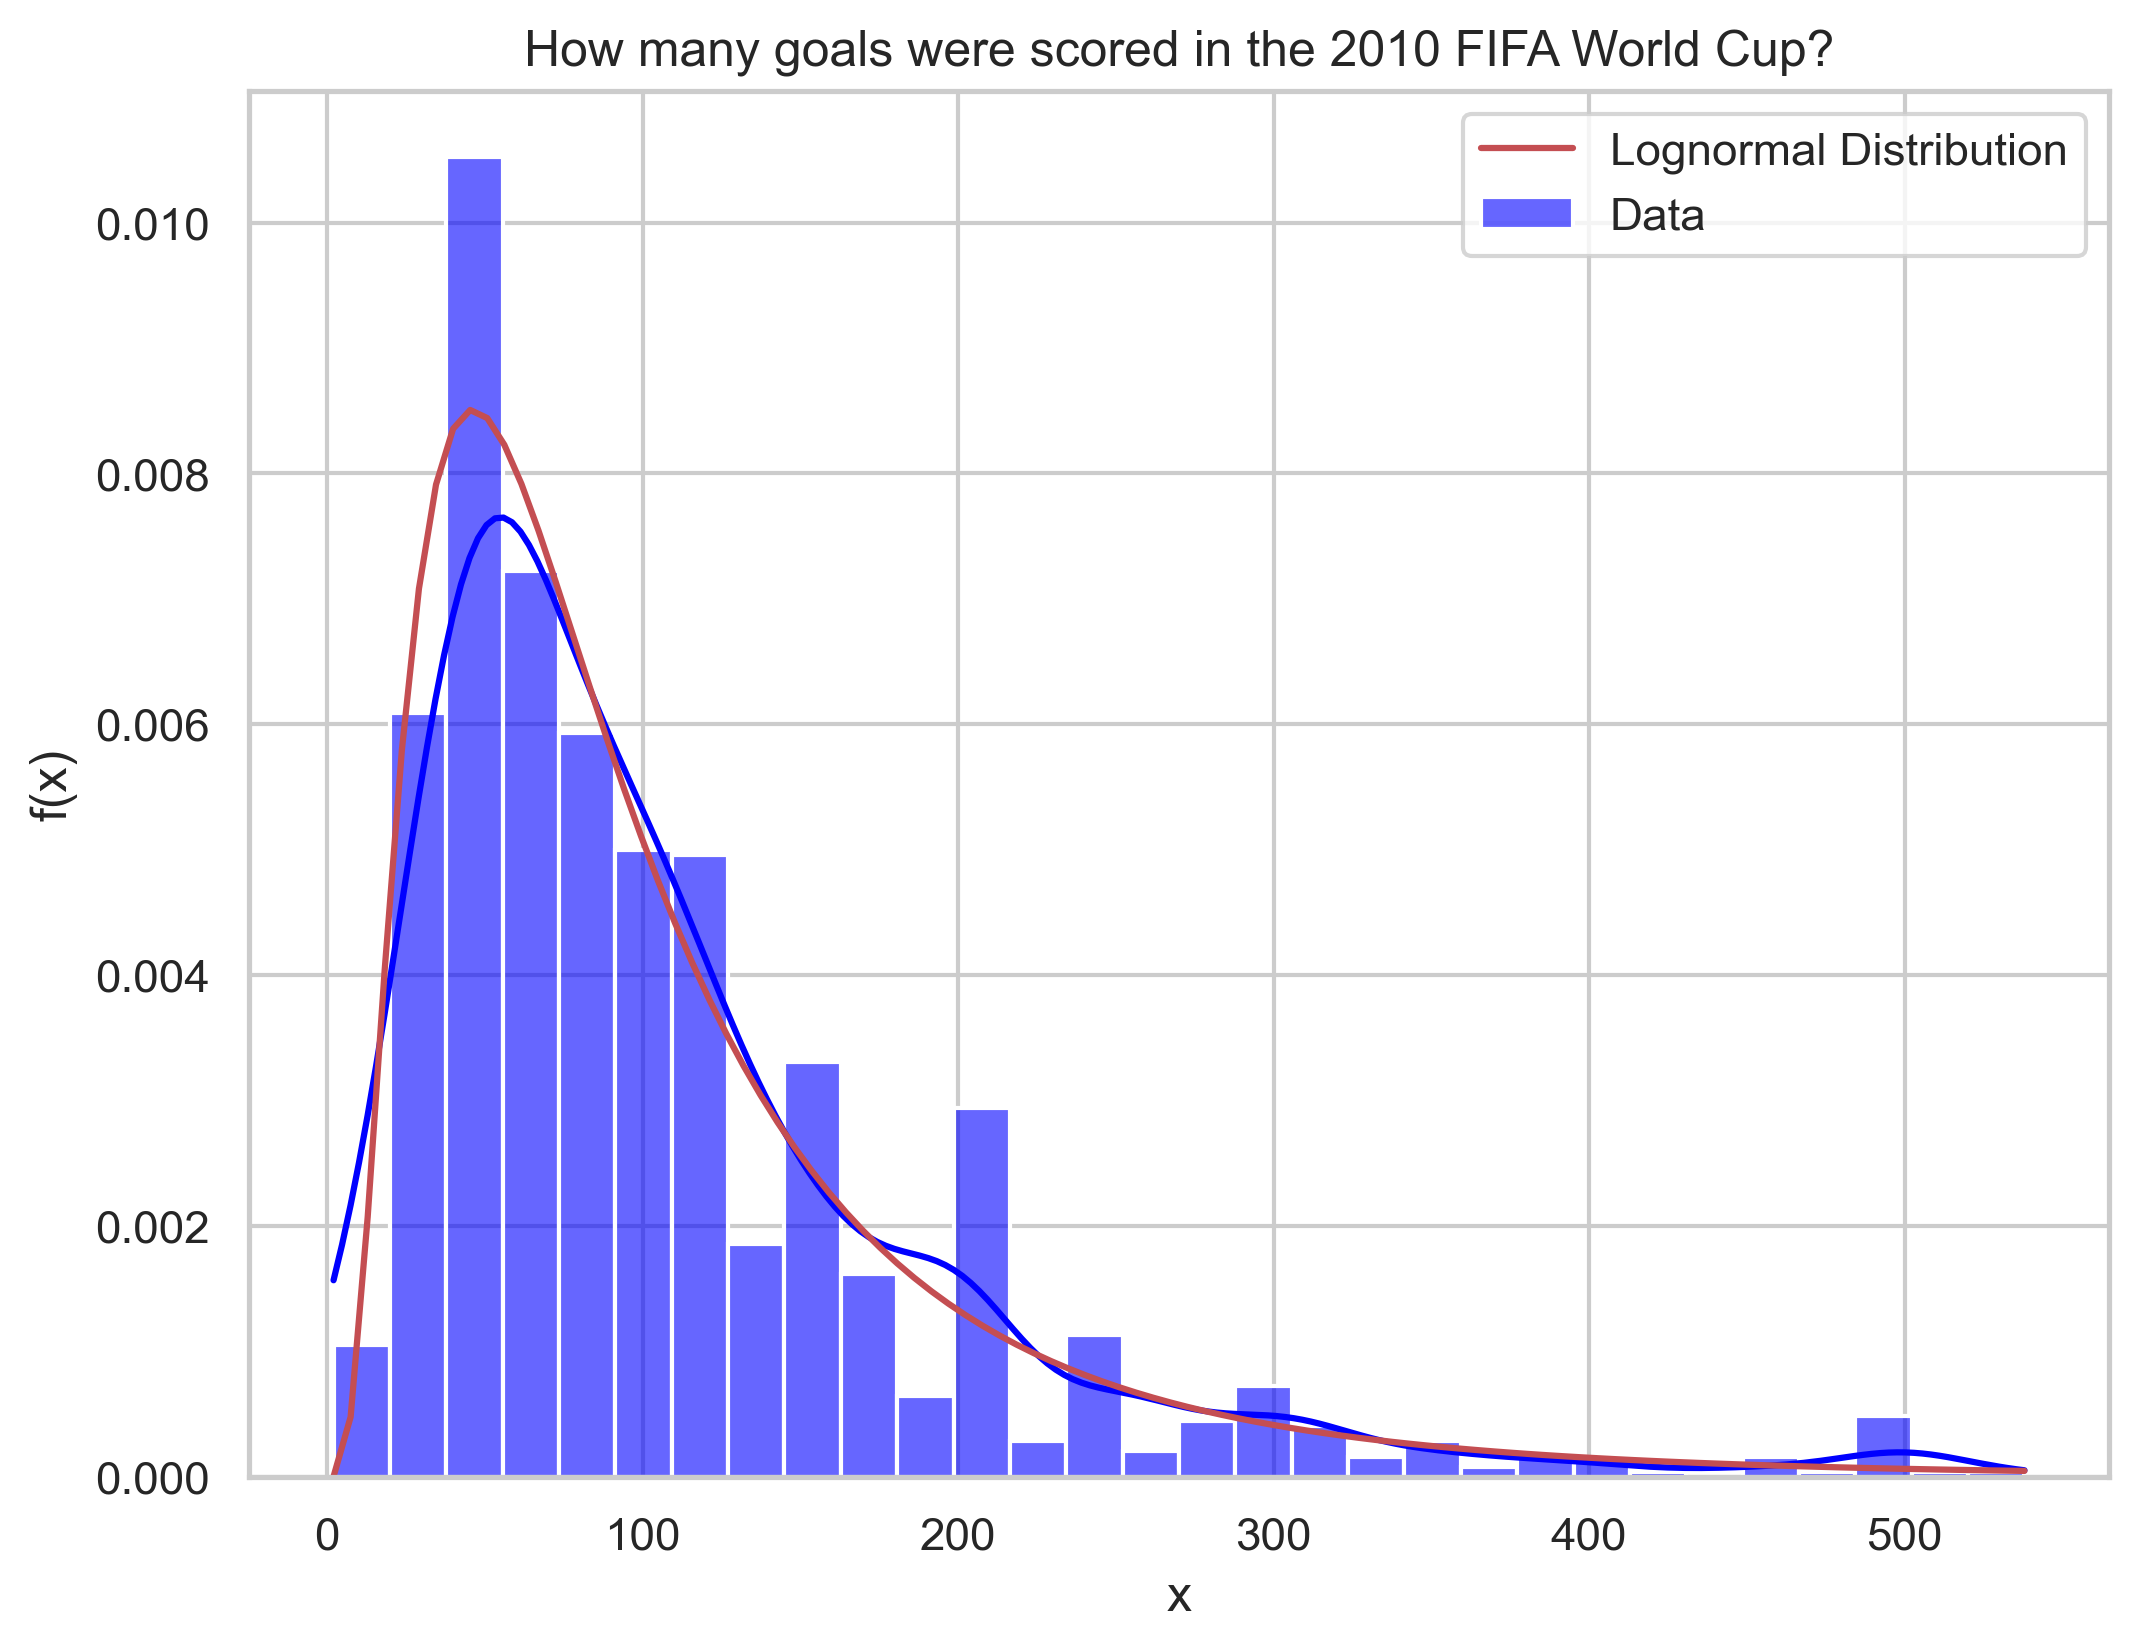
\includegraphics[width=0.8\textwidth]{figures/appendix_1/goals_distribution_log.png}
\caption{Distribución respuestas pregunta 1 y ajuste log-normal}
\end{figure}

\begin{figure}[h]
\centering
    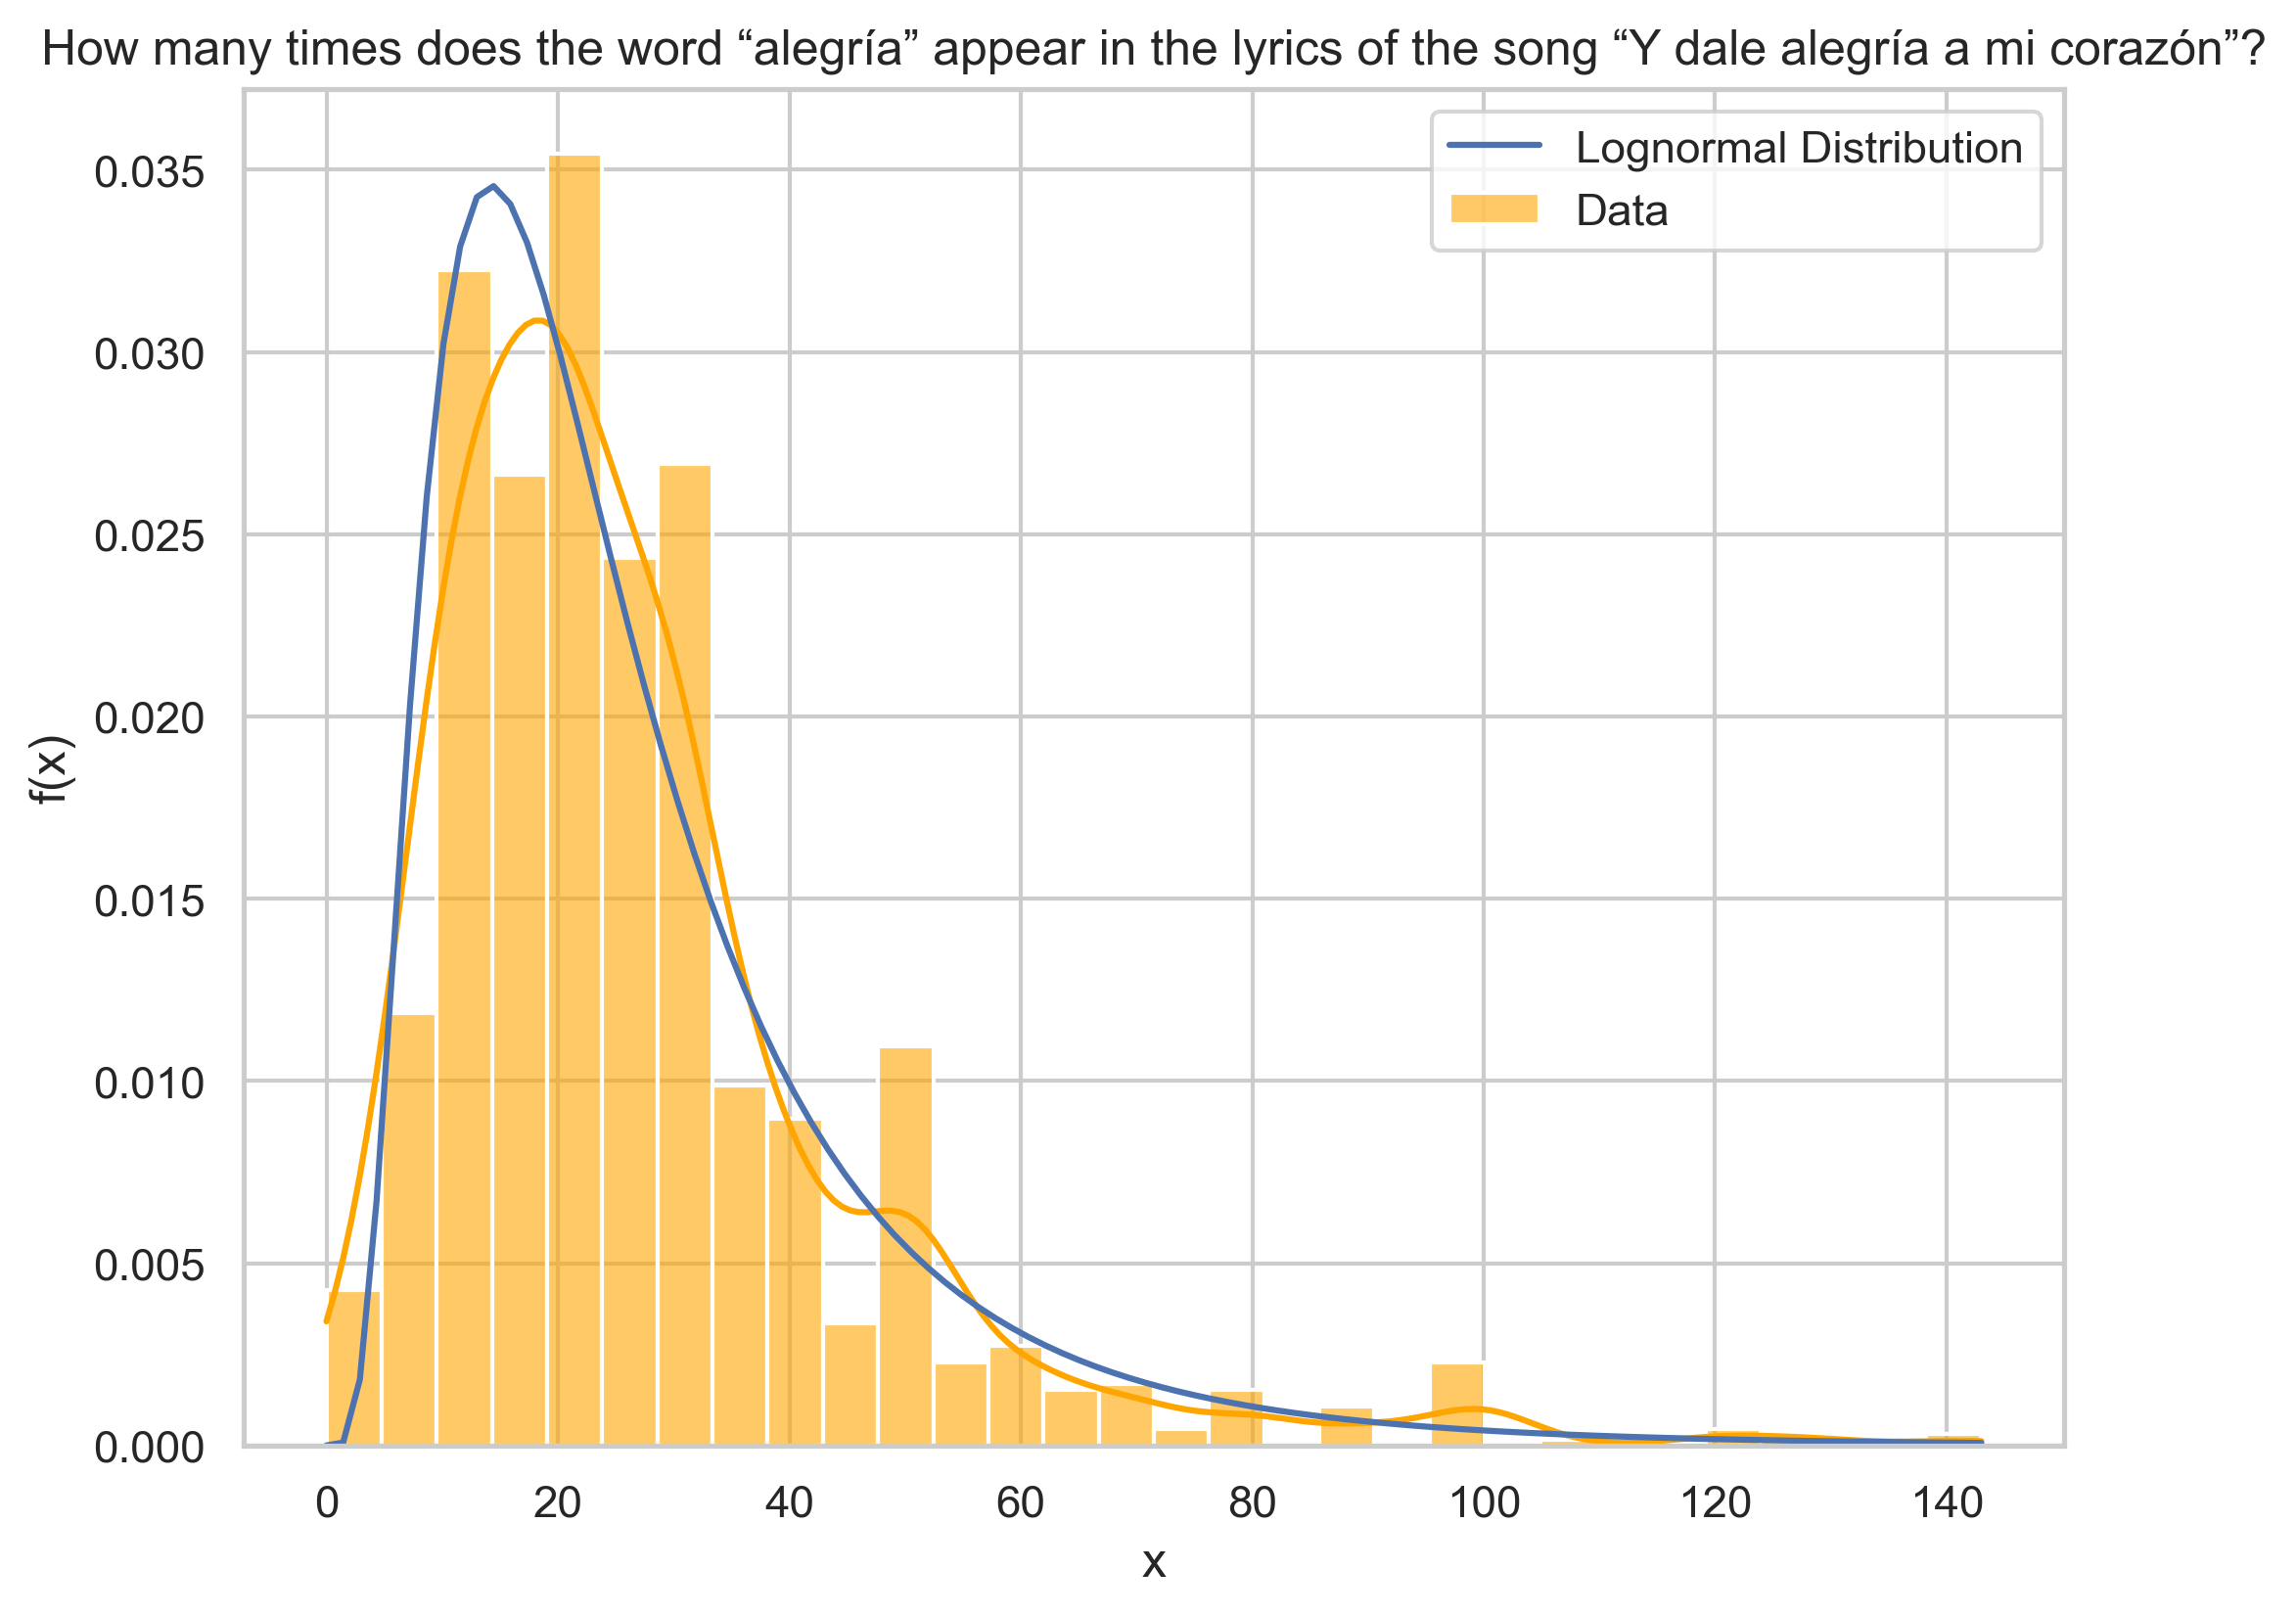
\includegraphics[width=0.8\textwidth]{figures/appendix_1/alegria_distribution_log.png}
\caption{Distribución respuestas pregunta 2 y ajuste log-normal}
\end{figure}

\begin{figure}[h]
\centering
    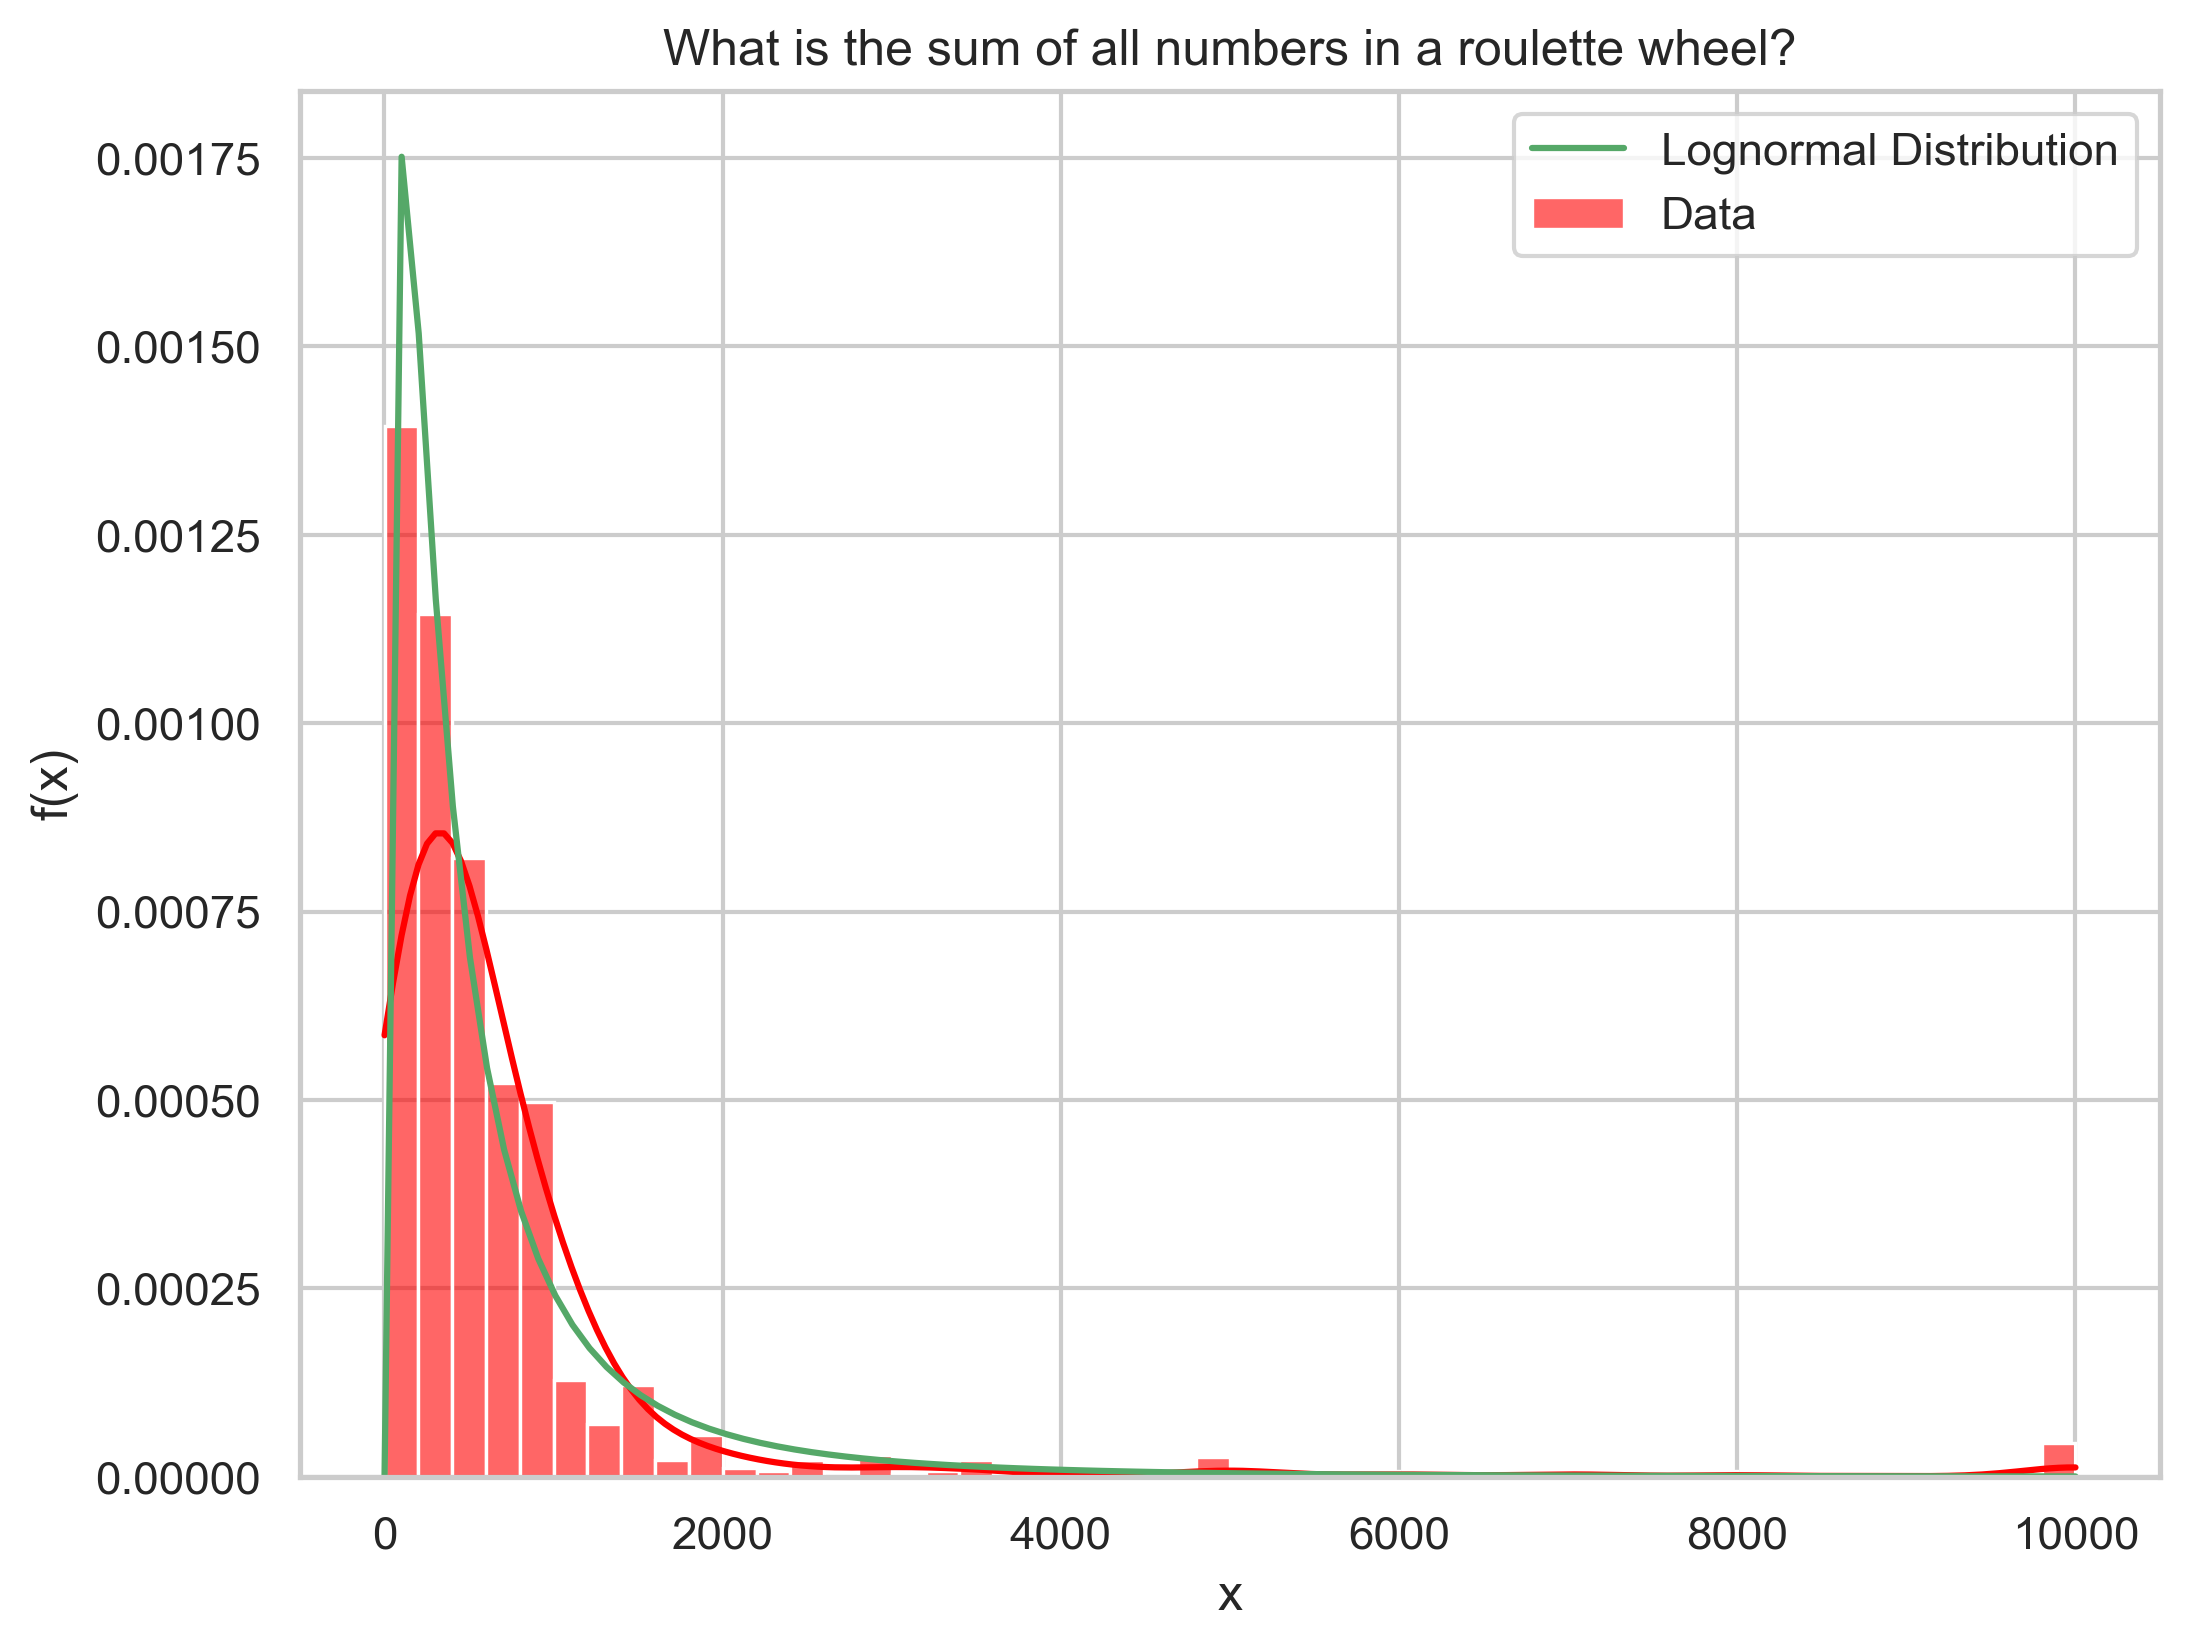
\includegraphics[width=0.8\textwidth]{figures/appendix_1/roullette_distribution_log.png}
\caption{Distribución respuestas pregunta 3 y ajuste log-normal}
\end{figure}

\begin{figure}[h]
\centering
    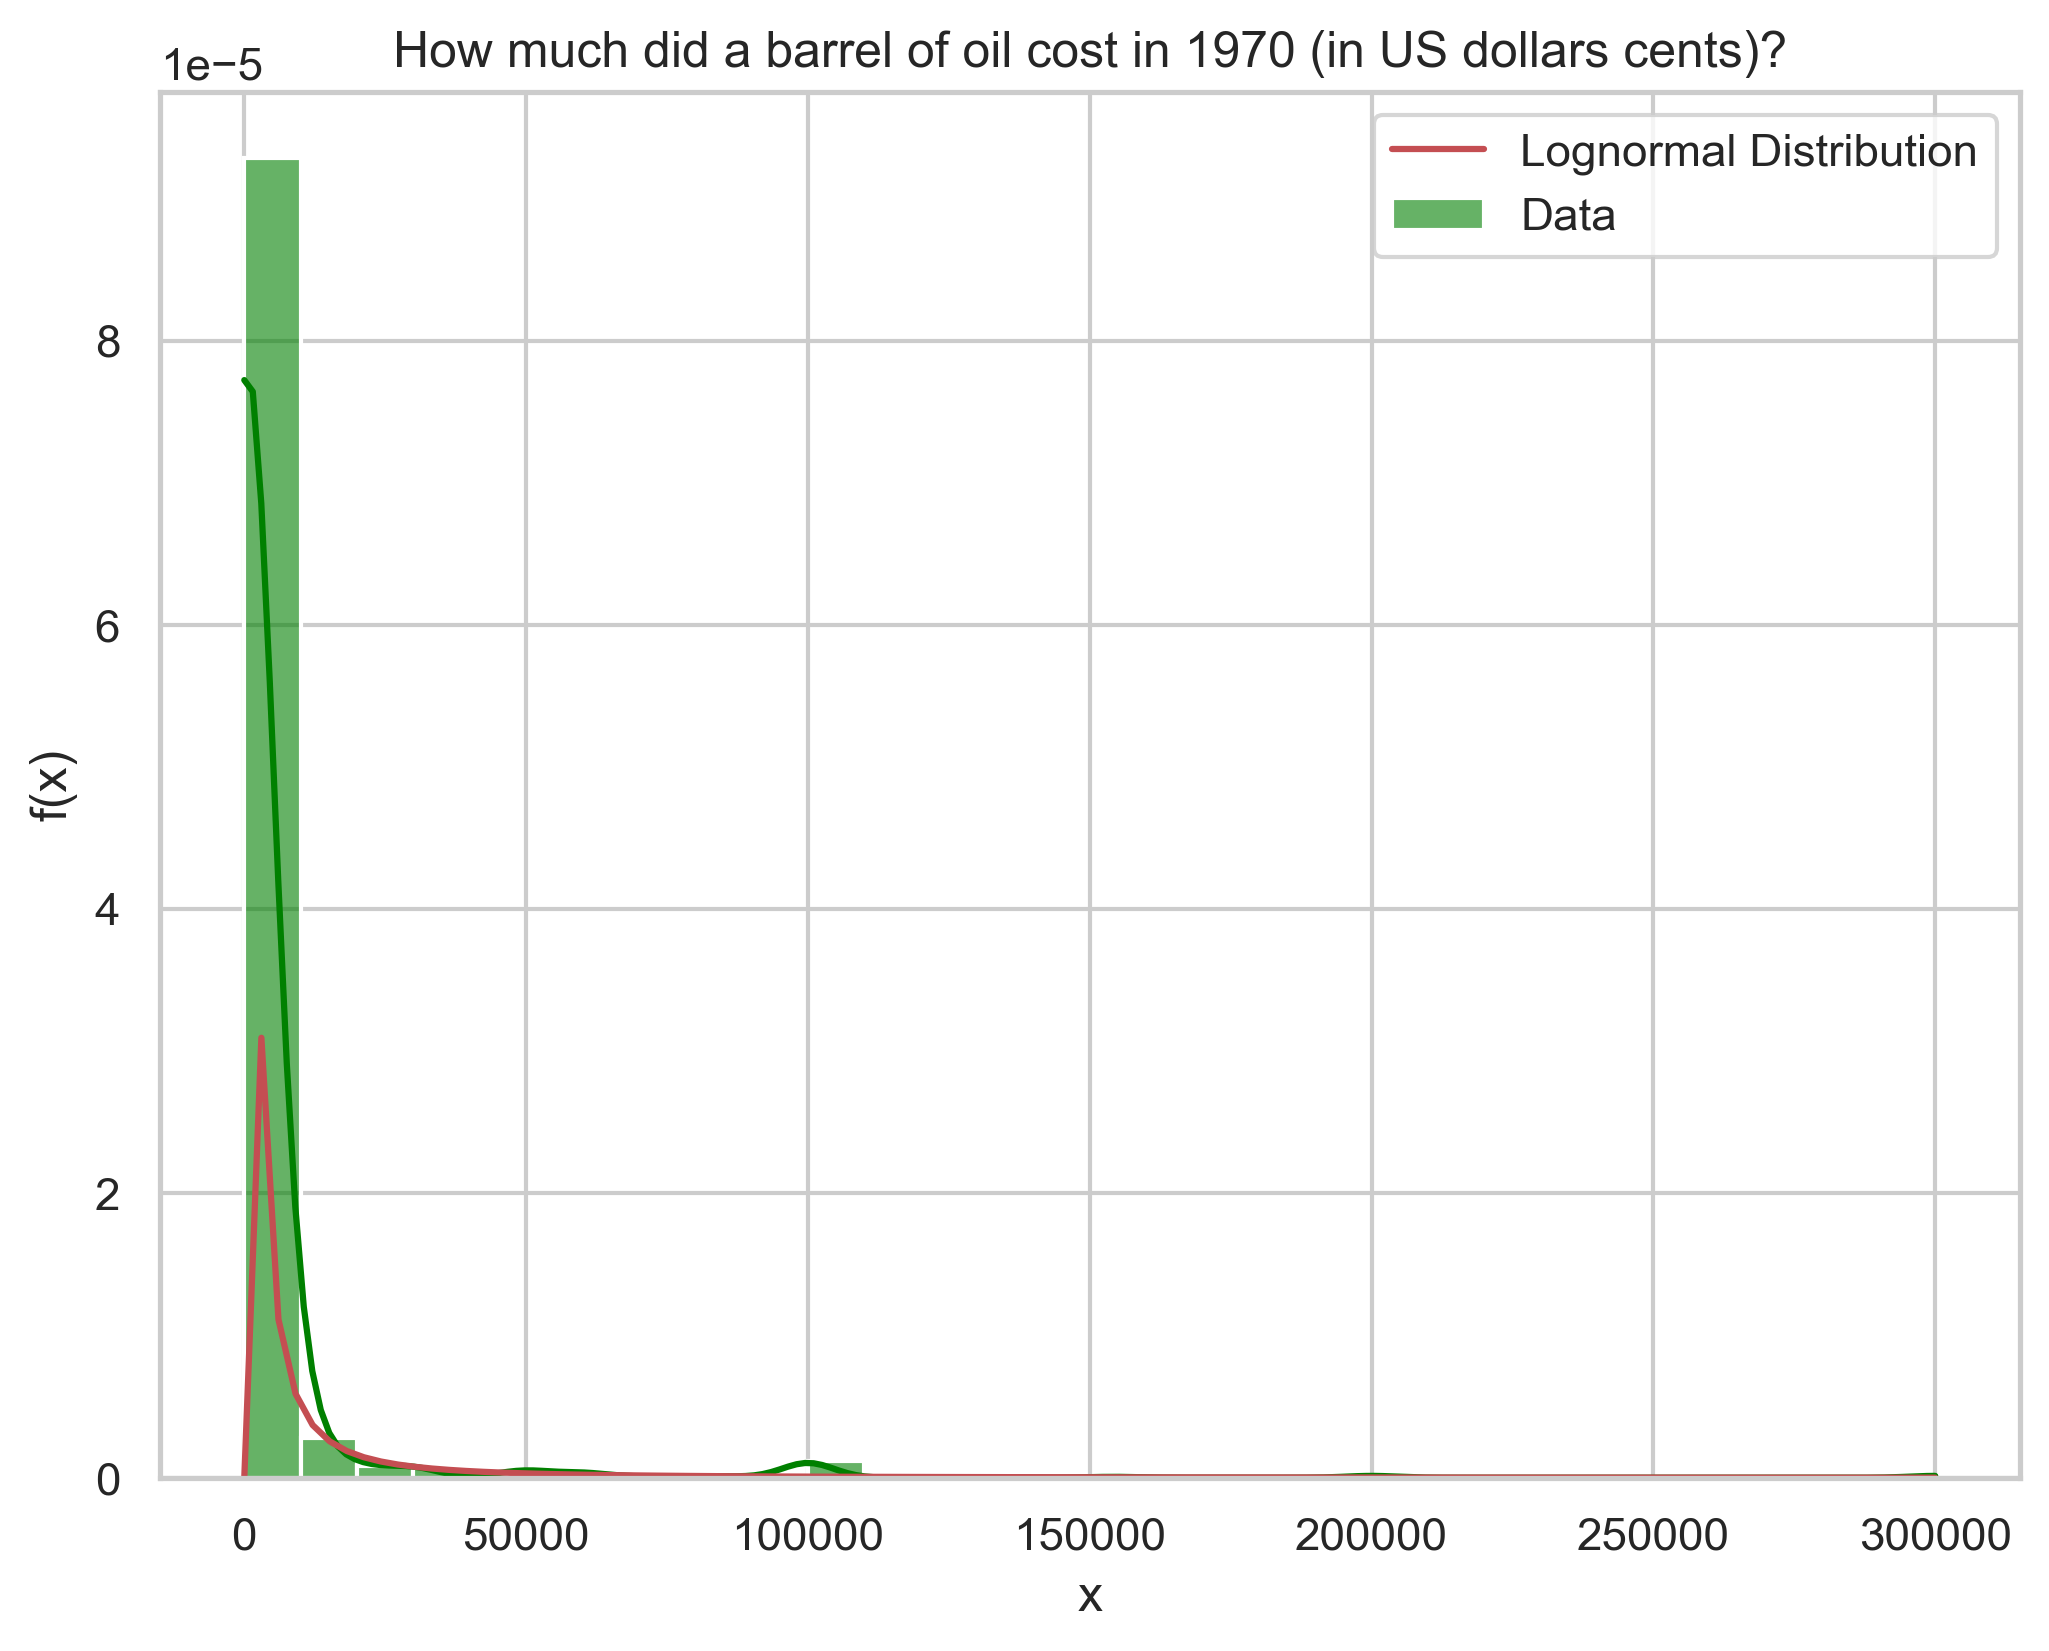
\includegraphics[width=0.8\textwidth]{figures/appendix_1/oil_distribution_log.png}
\caption{Distribución respuestas pregunta 4 y ajuste log-normal}
\end{figure}

% Ensure all figures are placed before moving to the next section
\FloatBarrier
 
\section*{2. Figuras distribución normal datos transformados}
 \label{appendix2}

 \begin{figure}[h]
\centering
    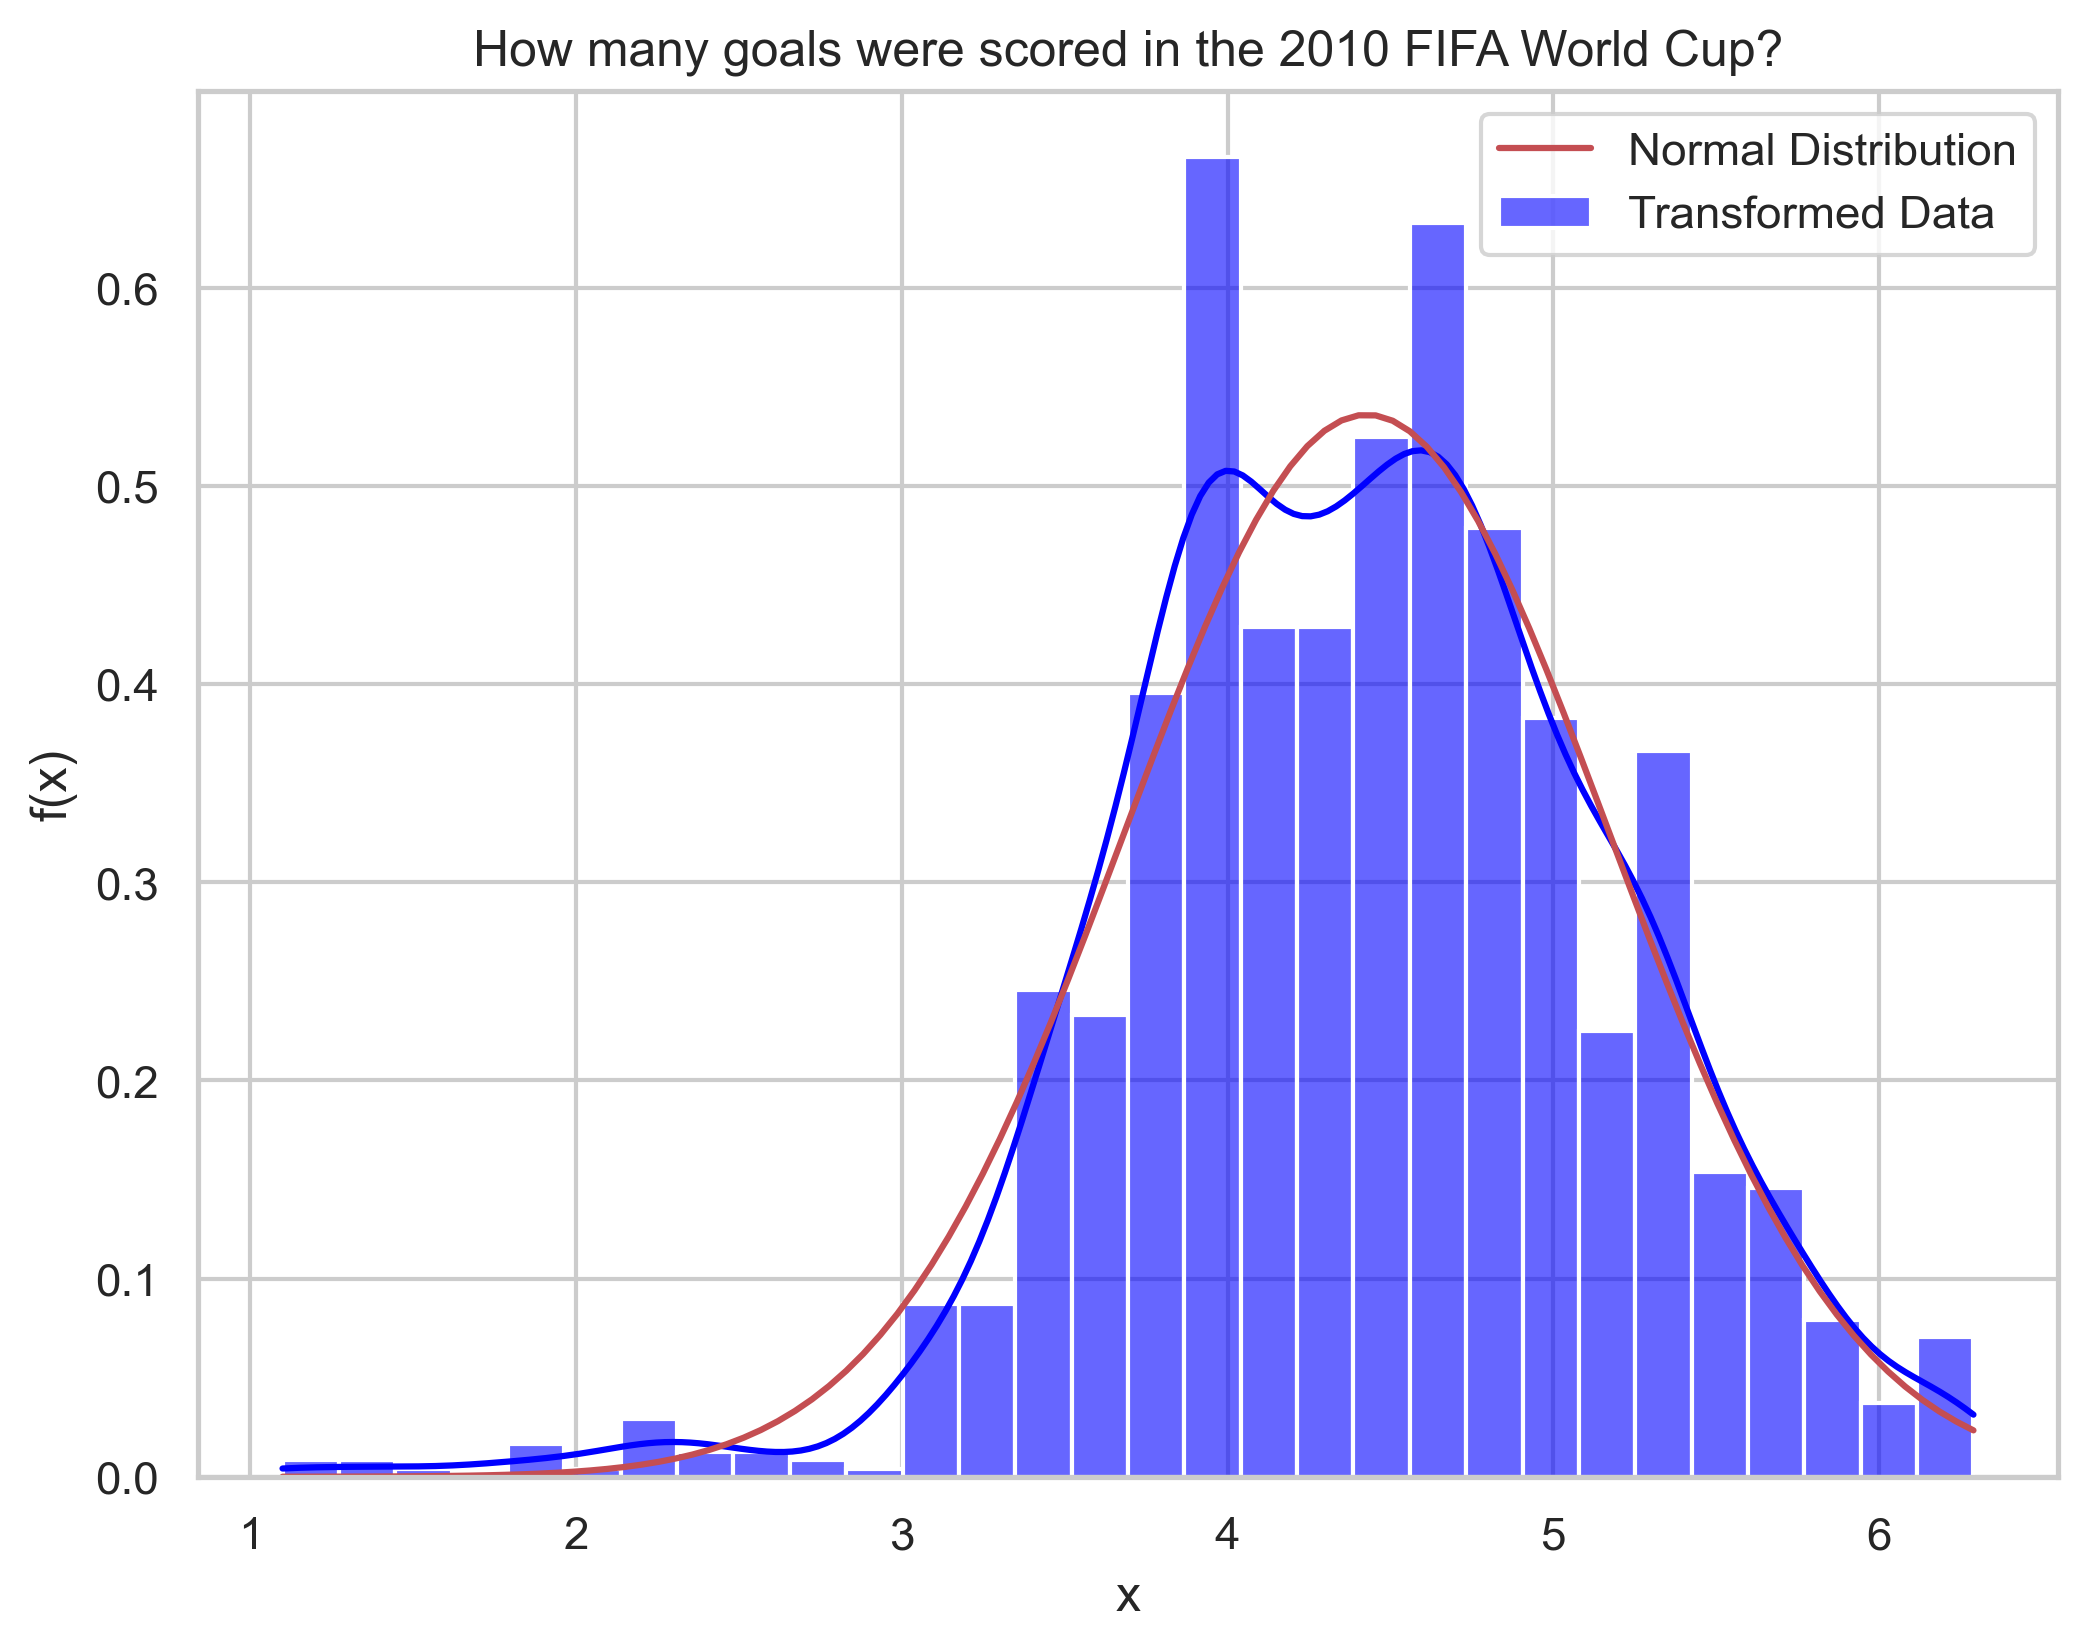
\includegraphics[width=0.8\textwidth]{figures/appendix_2/goals_distribution_normal.png}
\caption{Distribución respuestas pregunta 1 y ajuste normal}
\end{figure}

\begin{figure}[h]
\centering
    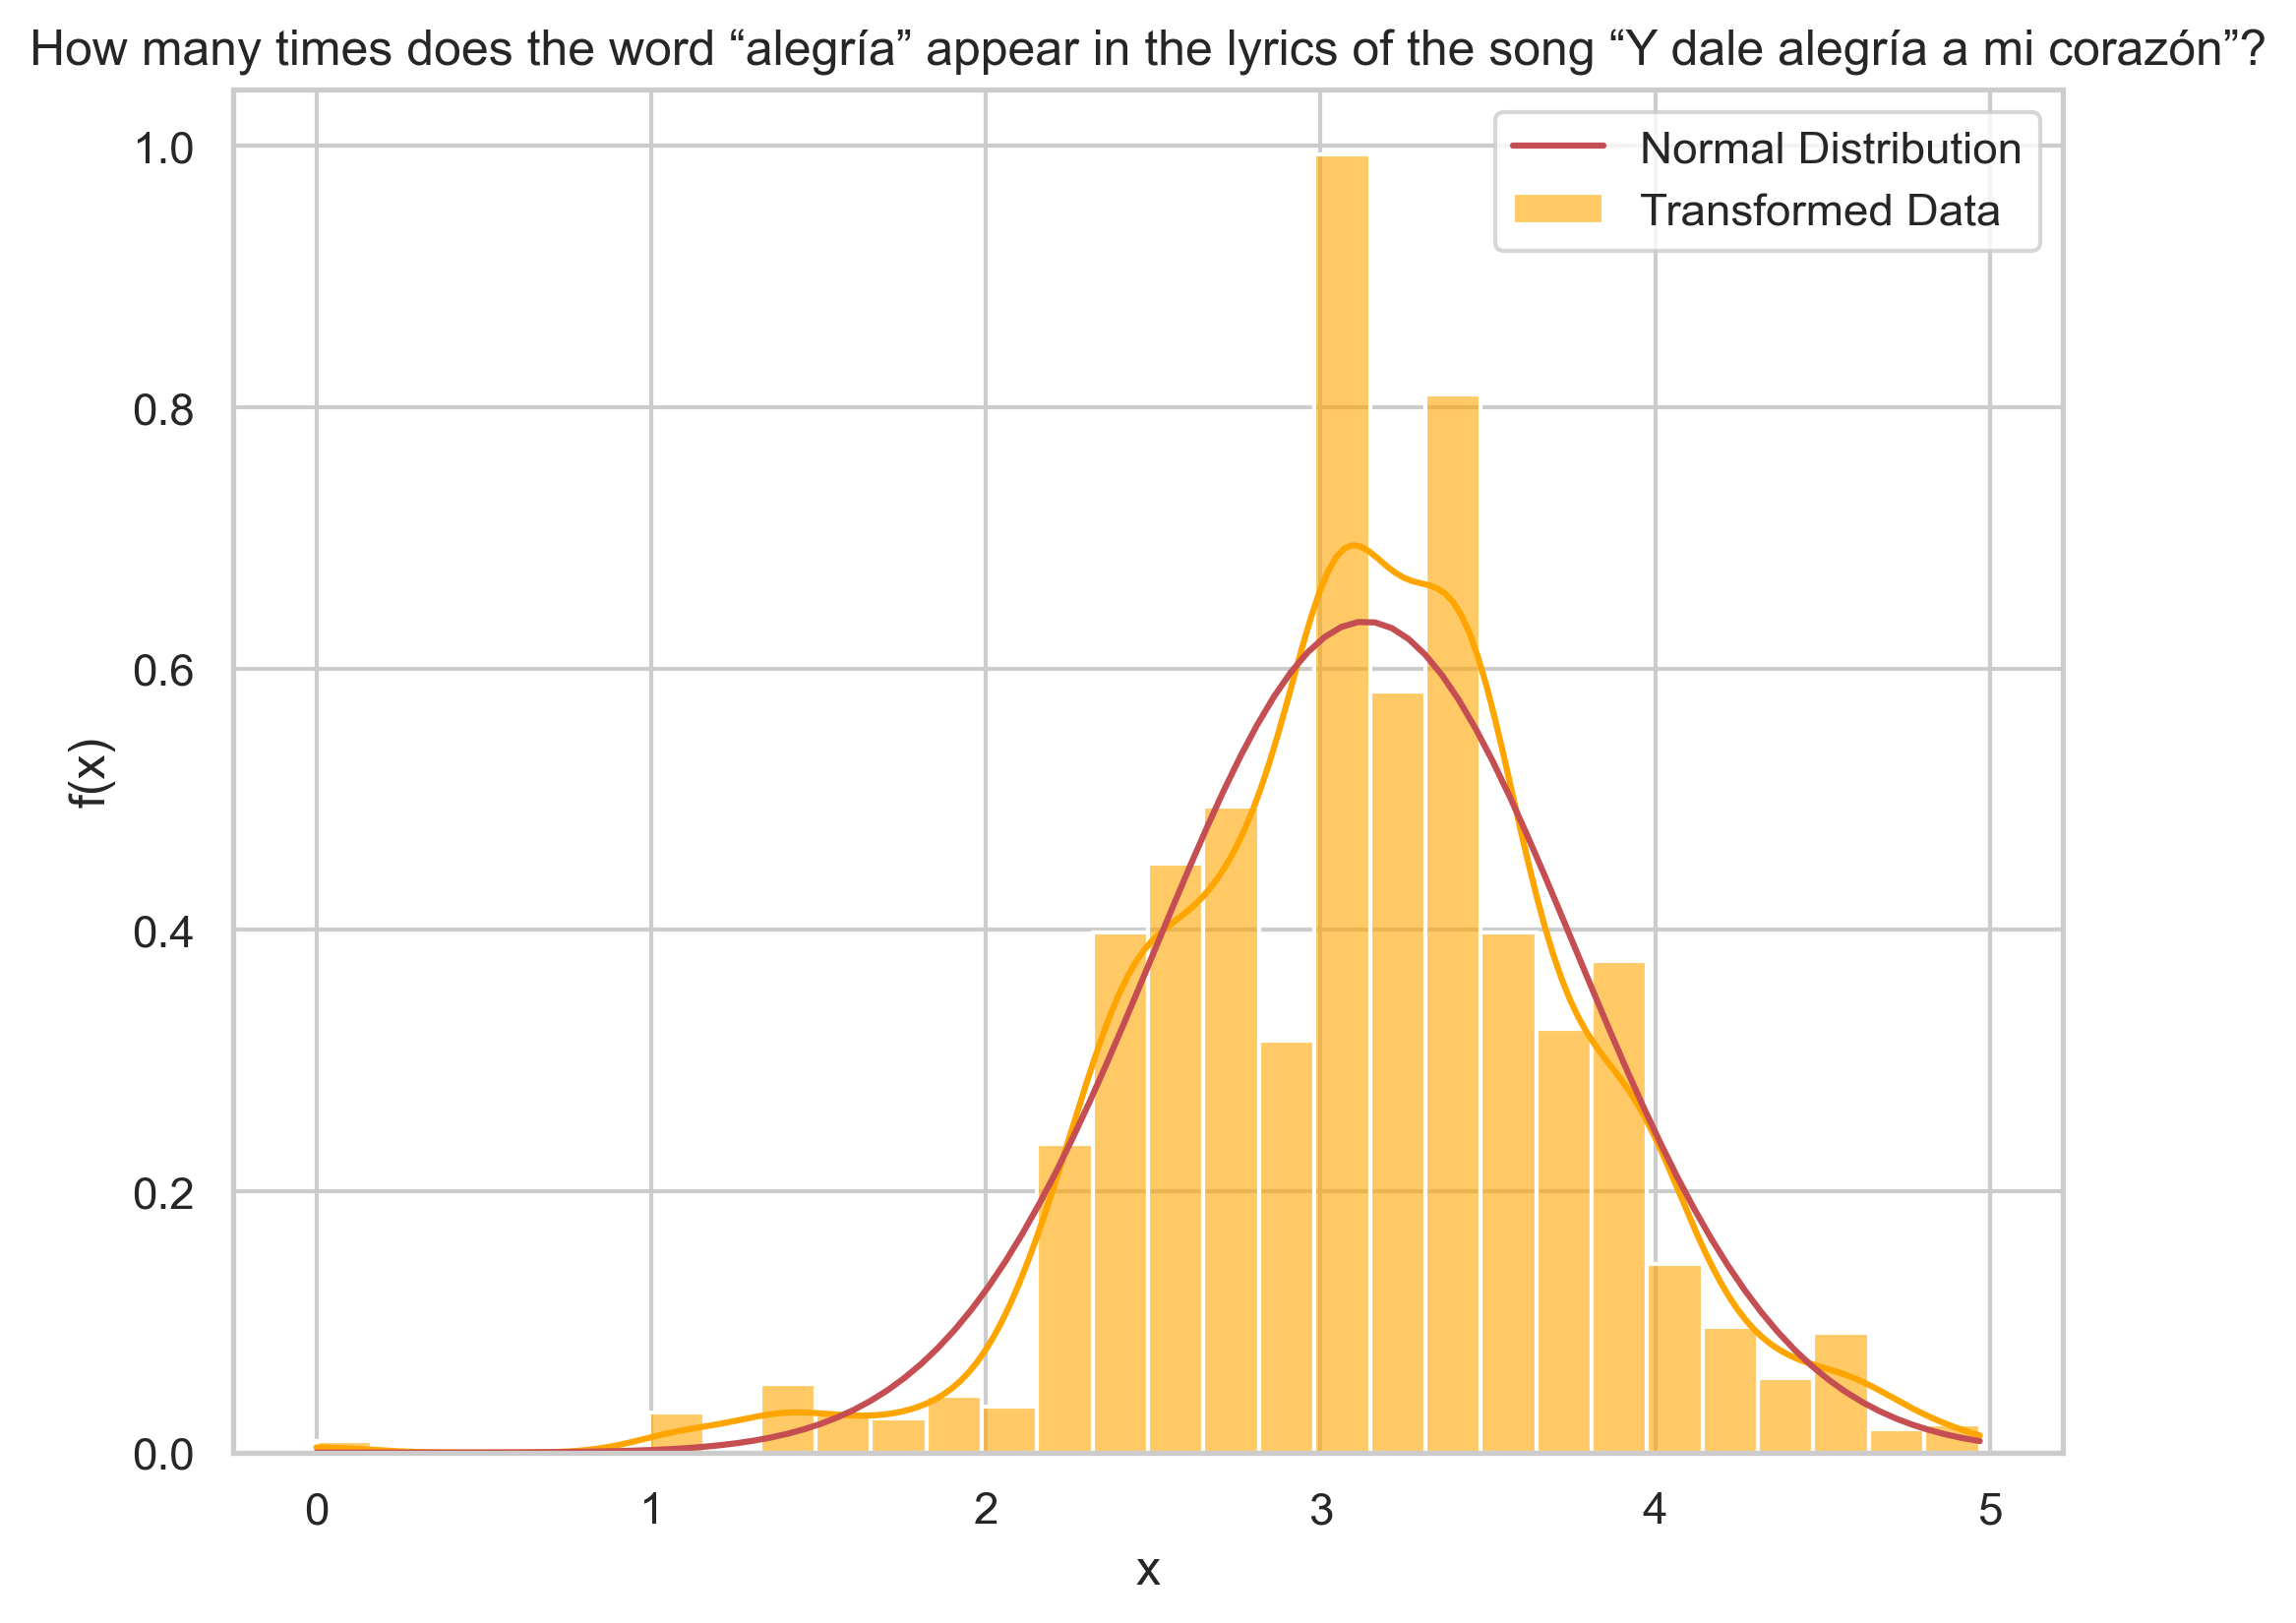
\includegraphics[width=0.8\textwidth]{figures/appendix_2/alegria_distribution_normal.png}
\caption{Distribución respuestas pregunta 2 y ajuste normal}
\end{figure}

\begin{figure}[h]
\centering
    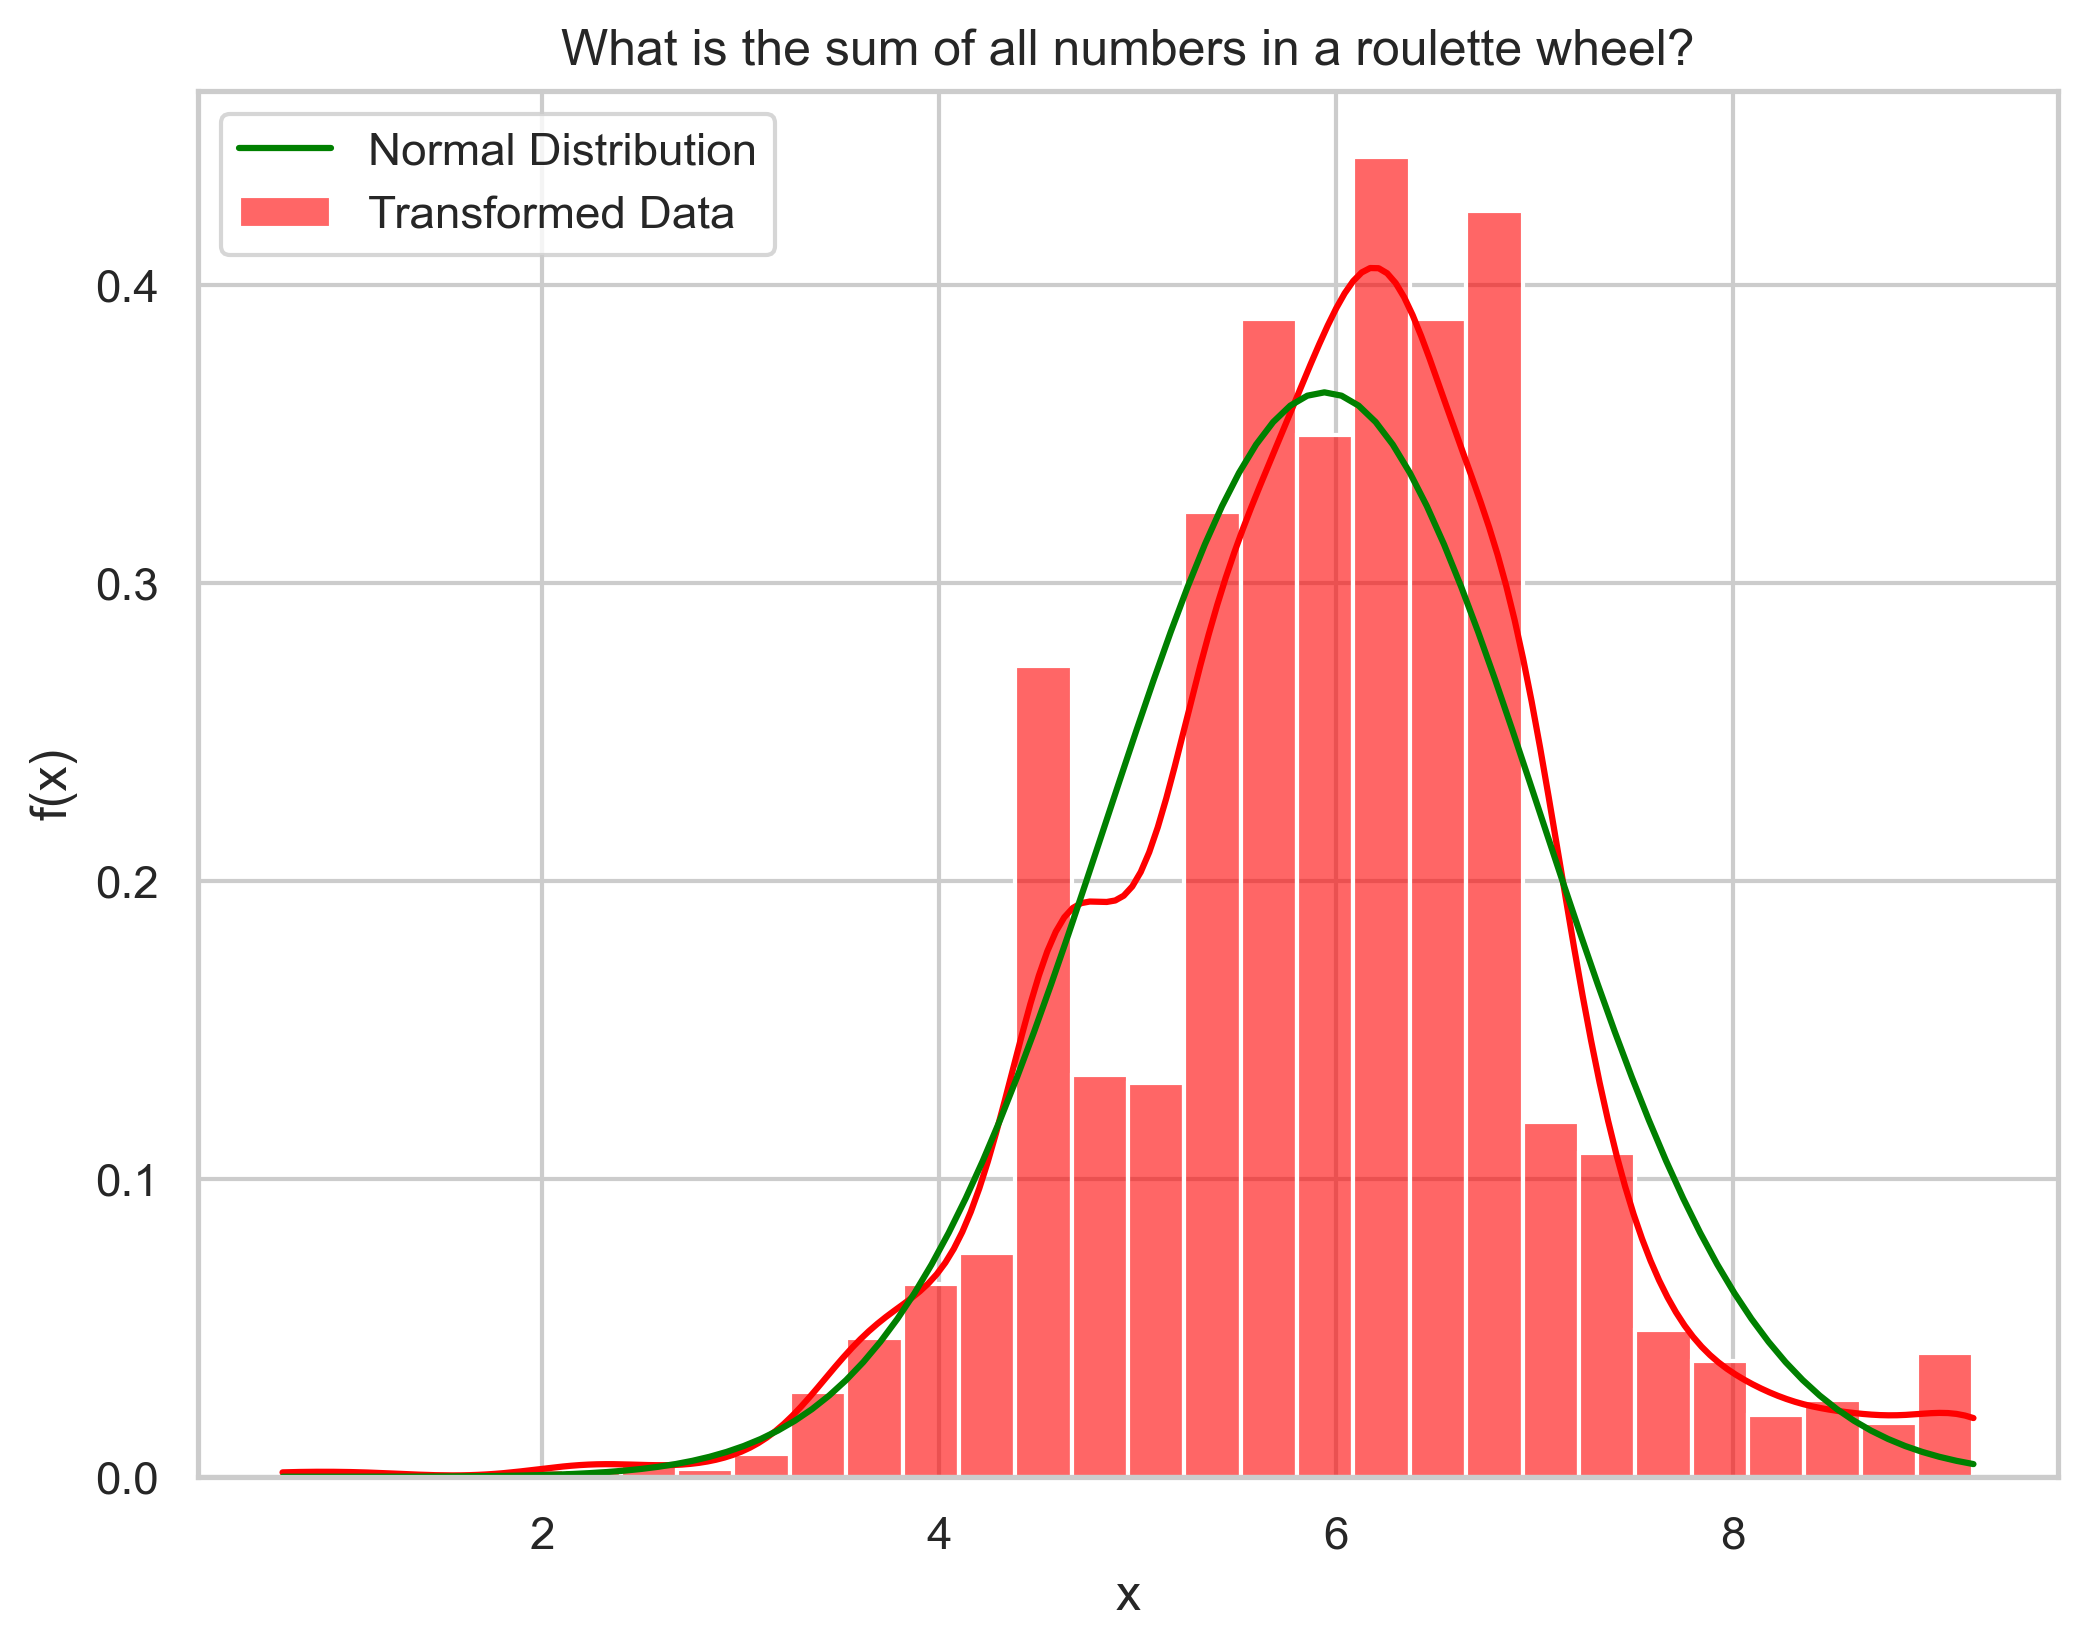
\includegraphics[width=0.8\textwidth]{figures/appendix_2/roullette_distribution_normal.png}
\caption{Distribución respuestas pregunta 3 y ajuste normal}
\end{figure}

\begin{figure}[h]
\centering
    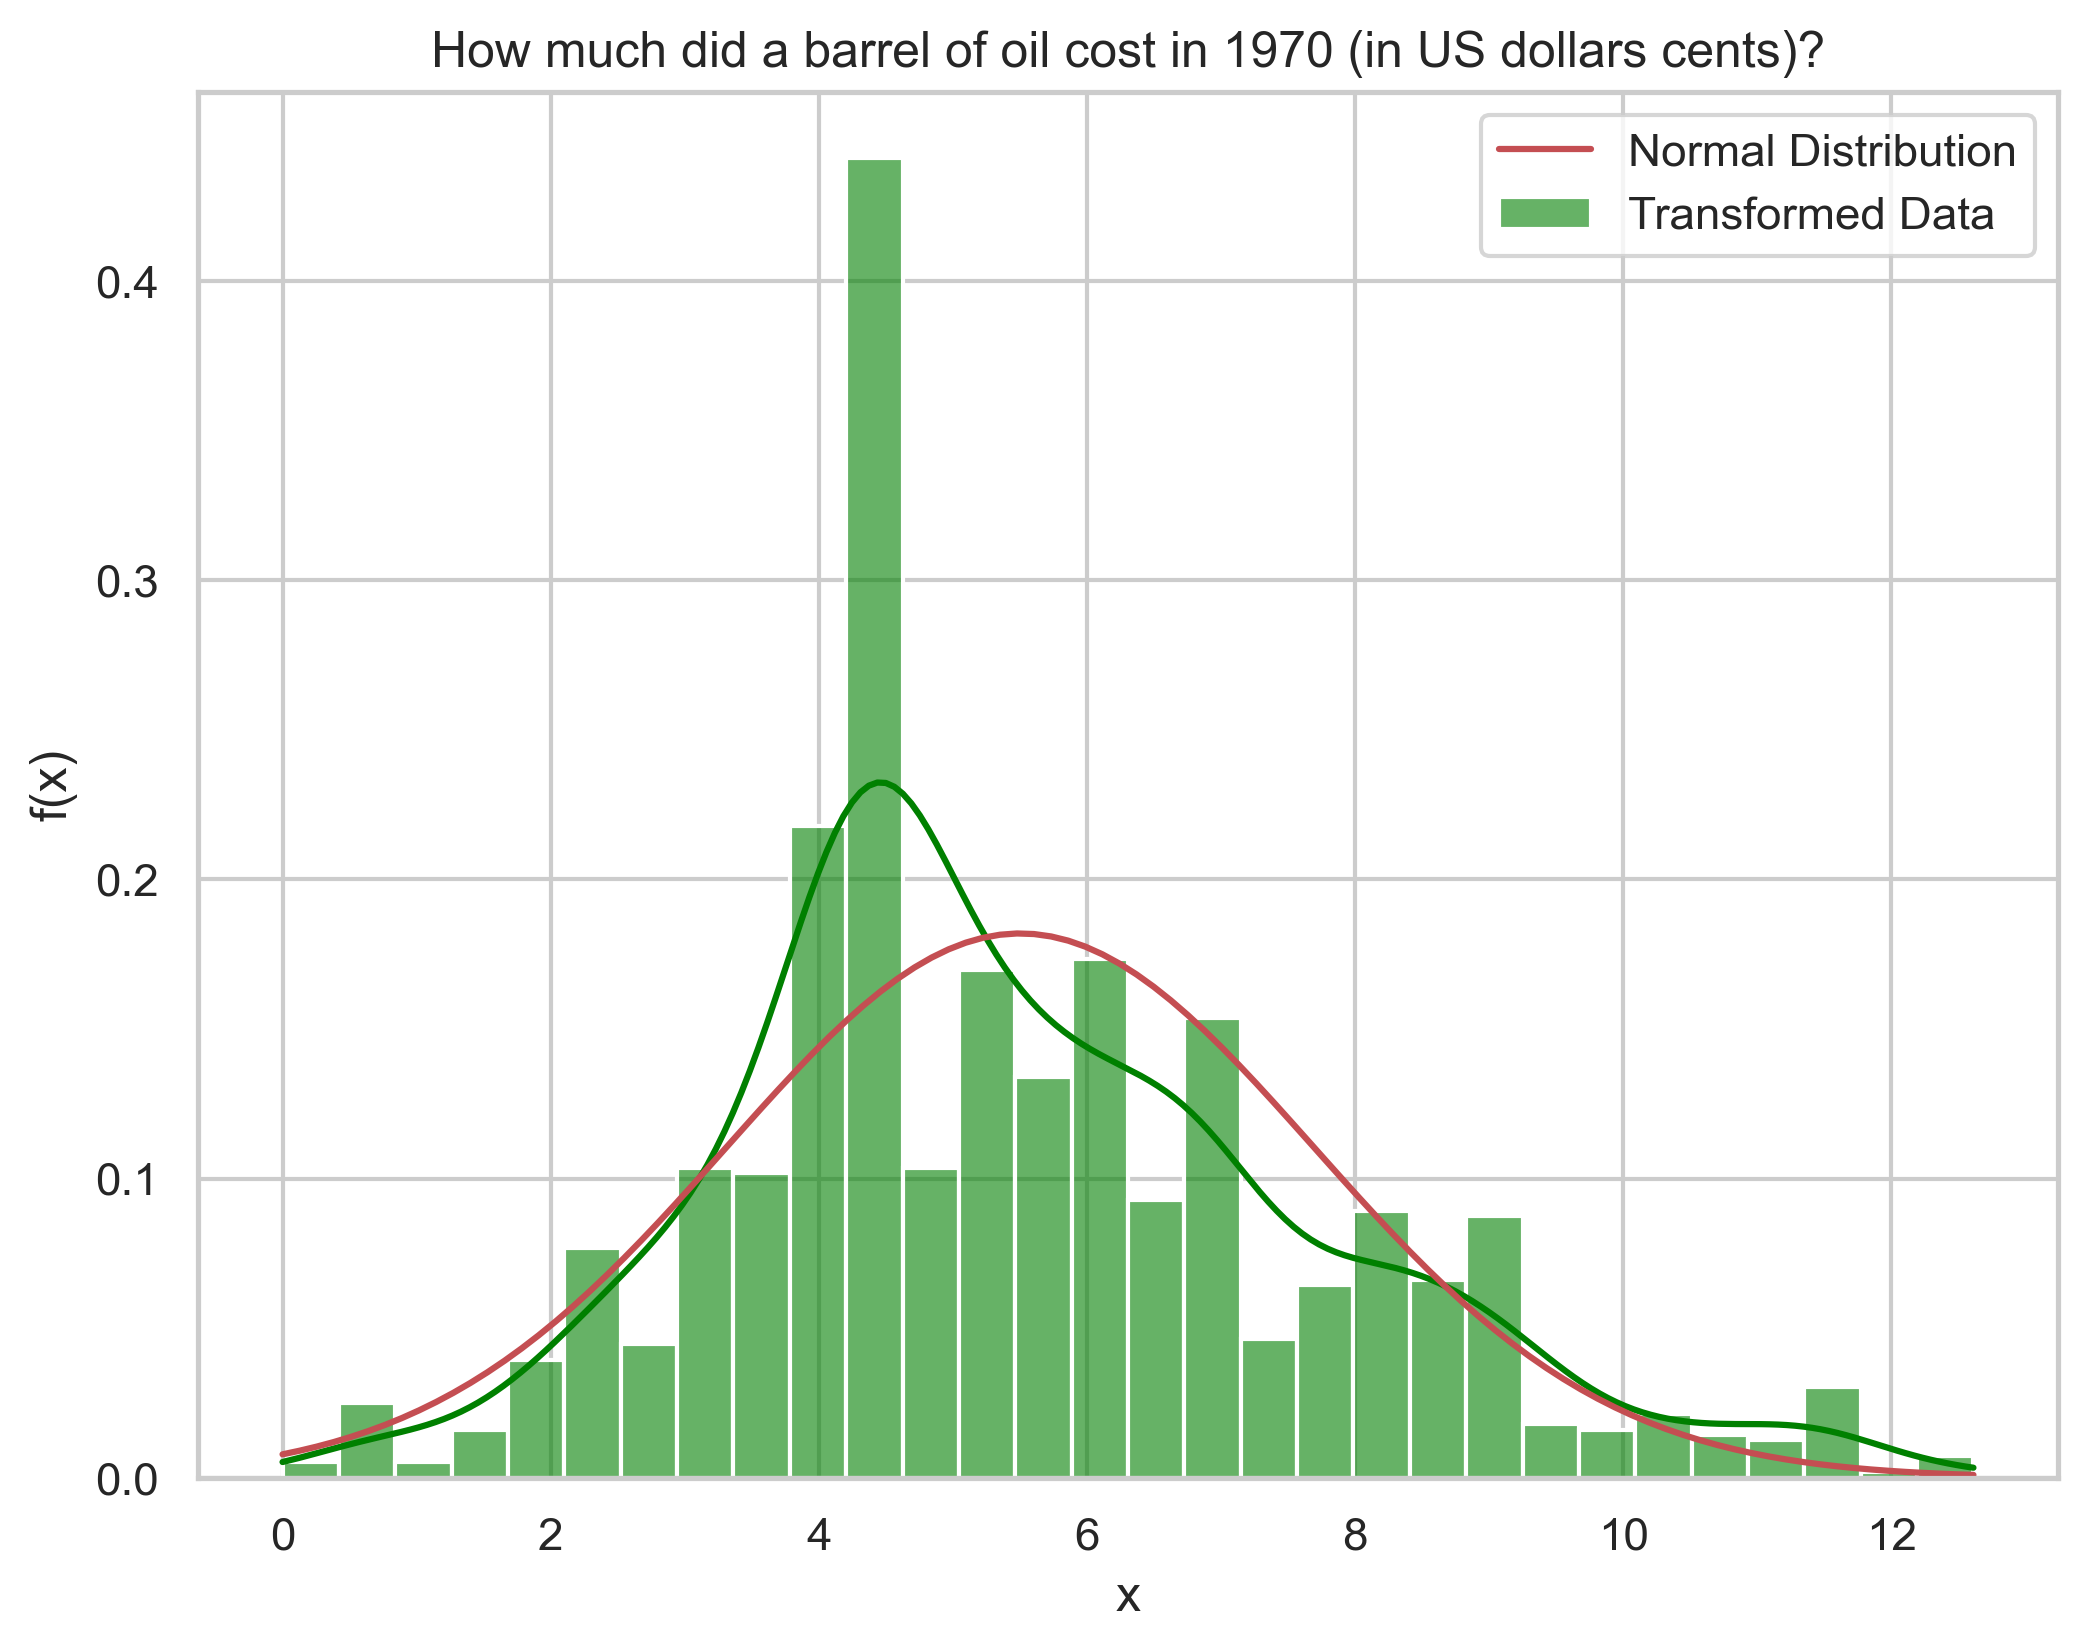
\includegraphics[width=0.8\textwidth]{figures/appendix_2/oil_distribution_normal.png}
\caption{Distribución respuestas pregunta 4 y ajuste normal}
\end{figure}

% Ensure all figures are placed before moving to the next section
\FloatBarrier
 
\section*{3. Tabla resultados test Shapiro-Wilk}
 \label{appendix3}
 
\begin{table}[h]
\centering
    \caption{Estadísticas y P-valores para diferentes preguntas}
    \label{tab:stats}
\begin{tabularx}{\textwidth}{l X X X}
\toprule
\textbf{Pregunta} & \textbf{Estadístico} & \textbf{P-valor} \\
\midrule
Goles    & $0.9839$ & $2.7140 \cdot 10^{-11}$ \\
Alegría  & $0.9833$ & $1.5691 \cdot 10^{-11}$ \\
Ruleta   & $0.9835$ & $2.5451 \cdot 10^{-11}$ \\
Petróleo & $0.9730$ & $4.7153 \cdot 10^{-15}$ \\
\bottomrule
\end{tabularx}
\end{table}

\FloatBarrier

\section*{4. Tabla datasets ordenados por nivel de aceptación}
 \label{appendix4}

\begin{table}[h]
\centering
    \caption{Proporción de aceptación de distribución por conjunto de datos}
\begin{tabularx}{\textwidth}{l X}
\toprule
\textbf{Nombre Dataset} & \textbf{Prop. aceptación} \\
\midrule
Carbon\_Emission.csv & 0.9485 \\
wind\_dataset.csv & 0.8360 \\
house\_8L.arff & 0.6954 \\
laptop.csv & 0.6143 \\
boston\_housing.arff & 0.5980 \\
abalone.csv & 0.5407 \\
salary\_football.csv & 0.4859 \\
Height.csv & 0.4171 \\
titanic\_fare.arff & 0.3817 \\
liver\_disorders.arff & 0.3623 \\
aerospace\_stock.arff & 0.3158 \\
Concrete\_Strength.csv & 0.3010 \\
kidney.arff & 0.25 \\
Metro\_Interstate\_Traffic\_Volume.csv & 0.2220 \\
weight.csv & 0.2098 \\
rainfall.arff & 0.1316 \\
flight\_price.csv & 0.1067 \\
medical\_costs.csv & 0.0784 \\
\bottomrule
\end{tabularx}
\end{table}

\FloatBarrier

\section*{5. Datasets seleccionados}
\label{appendix5}

Enlaces a los conjuntos de datos:

\begin{itemize}
    \item \href{https://www.openml.org/search?type=data&status=active&id=218}{House8L}
    \item \href{https://www.kaggle.com/datasets/fedesoriano/wind-speed-prediction-dataset}{Wind Speed}
    \item \href{https://www.kaggle.com/datasets/dumanmesut/individual-carbon-footprint-calculation}{Carbon Footprint}
    \item \href{https://www.kaggle.com/datasets/rodolfomendes/abalone-dataset}{Abalone}
    \item \href{https://www.openml.org/search?type=data&status=active&id=41539}{Rainfall}
    \item \href{https://www.kaggle.com/datasets/viveksharmar/flight-price-data}{Flight Price}
\end{itemize}

\section*{6. Setup entorno virtual}
\label{appendix6}

El paso por paso para configurar el entorno virtual se puede encontrar \textcolor{blue}{\href{https://github.com/fedeegiorgi/proyecto-final/blob/main/setup.pdf}{aquí}}.

\section*{7. Hiperparámetros definidos}
\label{appendix7}

\begin{table}[h]
\centering
    \caption{Hiperparámetros definidos para RF estándar por dataset.}
\begin{tabularx}{\textwidth}{l X}
\toprule
\textbf{Nombre Dataset} & \textbf{\texttt{max\_depth}} \\
\midrule
Carbon Footprint & 20 \\
House8L & 17 \\
Wind Speed & 12 \\
Abalone & 15 \\
Rainfall & 24 \\
Flight Price & 13 \\
\bottomrule
\end{tabularx}
\end{table}

\begin{table}[h]
\centering
    \caption{Hiperparámetros definidos para \texttt{IQRRandomForestRegressor} por dataset.}
\begin{tabularx}{\textwidth}{l X X X}
\toprule
\textbf{Nombre Dataset} & \textbf{\texttt{n\_estimators}} & \textbf{\texttt{group\_size}} & \textbf{\texttt{max\_depth}} \\
\midrule
Carbon Footprint & 150 & 3 & 20 \\
House8L & 150 & 3 & 32 \\
Wind Speed & 150 & 3 & 32 \\
Abalone & 150 & 3 & 12 \\
Rainfall & 150 & 3 & 21 \\
Flight Price & 150 & 3 & 13 \\
\bottomrule
\end{tabularx}
\end{table}

\begin{table}[h]
\centering
    \caption{Hiperparámetros definidos para \texttt{PercentileTrimmingRandomForestRegressor} por dataset.}
\begin{tabularx}{\textwidth}{l X X X X}
\toprule
\textbf{Nombre Dataset} & \textbf{\texttt{n\_estimators}} & \textbf{\texttt{group\_size}} & \textbf{\texttt{percentile}} &\textbf{\texttt{max\_depth}} \\
\midrule
Carbon Footprint & 150 & 50 & 2 & 44 \\
House8L & 150 & 50 & 2 & 40 \\
Wind Speed & 150 & 50 & 2 & 44 \\
Abalone & 150 & 50 & 2 & 12 \\
Rainfall & 150 & 50 & 2 & 23 \\
Flight Price & 150 & 50 & 2 & 13 \\
\bottomrule
\end{tabularx}
\end{table}

\begin{table}[h]
\centering
    \caption{Hiperparámetros definidos para \texttt{OOBRandomForestRegressor} por dataset.}
\begin{tabularx}{\textwidth}{l X X X}
\toprule
\textbf{Nombre Dataset} & \textbf{\texttt{n\_estimators}} & \textbf{\texttt{group\_size}} & \textbf{\texttt{max\_depth}} \\
\midrule
Carbon Footprint & 180 & 3 & 17 \\
House8L & 180 & 3 & 17 \\
Wind Speed & 180 & 3 & 19 \\
Abalone & 180 & 3 & 10 \\
Rainfall & 180 & 3 & 23 \\
Flight Price & 180 & 3 & 13 \\
\bottomrule
\end{tabularx}
\end{table}

\begin{table}[h]
\centering
    \caption{Hiperparámetros definidos para \texttt{OOBPlusIQRRandomForestRegressor} por dataset.}
\begin{tabularx}{\textwidth}{l X X X}
\toprule
\textbf{Nombre Dataset} & \textbf{\texttt{n\_estimators}} & \textbf{\texttt{group\_size}} & \textbf{\texttt{max\_depth}} \\
\midrule
Carbon Footprint & 180 & 3 & 21 \\
House8L & 180 & 3 & 42 \\
Wind Speed & 180 & 3 & 14 \\
Abalone & 180 & 3 & 10 \\
Rainfall & 180 & 3 & 23 \\
Flight Price & 180 & 3 & 13 \\
\bottomrule
\end{tabularx}
\end{table}

\begin{table}[h]
\centering
    \caption{Hiperparámetros definidos para \texttt{FirstSplitCombinerRandomForestRegressor} por dataset.}
\begin{tabularx}{\textwidth}{l X X X}
\toprule
\textbf{Nombre Dataset} & \textbf{\texttt{n\_estimators}} & \textbf{\texttt{group\_size}} & \textbf{\texttt{max\_features}} \\
\midrule
Carbon Footprint & 100 & 10 & $log_2$ \\
House8L & 100 & 10 & $log_2$ \\
Wind Speed & 100 & 10 & $log_2$ \\
Abalone & 100 & 10 & $log_2$ \\
Rainfall & 100 & 10 & $log_2$ \\
Flight Price & 100 & 10 & $log_2$ \\
\bottomrule
\end{tabularx}
\end{table}

\begin{table}[h]
\centering
    \caption{Hiperparámetros definidos para \texttt{SharedKnowledgeRandomForestRegressor} por dataset.}
\begin{tabularx}{\textwidth}{l X X X X}
\toprule
\textbf{Nombre Dataset} & \textbf{\texttt{n\_estimators}} & \textbf{\texttt{group\_size}} & \textbf{\texttt{initial\_max\_depth}} &\textbf{\texttt{max\_depth}} \\
\midrule
Carbon Footprint & 280 & 7 & 14 & 20 \\
House8L & 280 & 7 & 14 & 23 \\
Wind Speed & 280 & 7 & 14 & 25 \\
Abalone & 280 & 7 & 14 & 23 \\
Rainfall & 280 & 7 & 14 & 39 \\
Flight Price & 280 & 7 & 14 & 20 \\
\bottomrule
\end{tabularx}
\end{table}

\FloatBarrier

\section*{8. Tablas comparación de modelos cross-validation}
\label{appendix8}

\begin{table}[h]
\centering
\begin{tabular}{|l|c|c|c|}
\hline
Model & Fold & MSE & Rank \\ \hline
\textcolor[HTML]{b33dc6}{OOBRandomForestRegressor} & 6 & 219626.05 & 1 \\ \hline
\textcolor[HTML]{ede15b}{OOBPlusIQRRandomForestRegressor} & 6 & 220018.76 & 2 \\ \hline
\textcolor[HTML]{27aeef}{IQRRandomForestRegressor} & 6 & 221685.1 & 3 \\ \hline
\textcolor[HTML]{ef9b20}{SharedKnowledgeRandomForestRegressor} & 6 & 221735.16 & 4 \\ \hline
\textcolor[HTML]{f46a9b}{PercentileTrimmingRandomForestRegressor} & 6 & 223235.21 & 5 \\ \hline
\textcolor[HTML]{f46a9b}{PercentileTrimmingRandomForestRegressor} & 3 & 223237.69 & 6 \\ \hline
\textcolor[HTML]{87bc45}{RandomForestRegressor} & 6 & 223837.16 & 7 \\ \hline
\textcolor[HTML]{27aeef}{IQRRandomForestRegressor} & 3 & 223963.58 & 8 \\ \hline
\textcolor[HTML]{87bc45}{RandomForestRegressor} & 3 & 224435.49 & 9 \\ \hline
\textcolor[HTML]{ede15b}{OOBPlusIQRRandomForestRegressor} & 3 & 224960.73 & 10 \\ \hline
\textcolor[HTML]{b33dc6}{OOBRandomForestRegressor} & 3 & 225963.59 & 11 \\ \hline
\textcolor[HTML]{b33dc6}{OOBRandomForestRegressor} & 1 & 226485.15 & 12 \\ \hline
\textcolor[HTML]{ef9b20}{SharedKnowledgeRandomForestRegressor} & 1 & 227177.42 & 13 \\ \hline
\textcolor[HTML]{87bc45}{RandomForestRegressor} & 1 & 227370.46 & 14 \\ \hline
\textcolor[HTML]{ef9b20}{SharedKnowledgeRandomForestRegressor} & 3 & 227639.59 & 15 \\ \hline
\textcolor[HTML]{ede15b}{OOBPlusIQRRandomForestRegressor} & 1 & 230364.45 & 16 \\ \hline
\textcolor[HTML]{27aeef}{IQRRandomForestRegressor} & 1 & 231118.59 & 17 \\ \hline
\textcolor[HTML]{f46a9b}{PercentileTrimmingRandomForestRegressor} & 1 & 231349.01 & 18 \\ \hline
\textcolor[HTML]{ede15b}{OOBPlusIQRRandomForestRegressor} & 7 & 234270.29 & 19 \\ \hline
\textcolor[HTML]{ef9b20}{SharedKnowledgeRandomForestRegressor} & 7 & 234414.21 & 20 \\ \hline
\textcolor[HTML]{27aeef}{IQRRandomForestRegressor} & 7 & 235863.45 & 21 \\ \hline
\textcolor[HTML]{b33dc6}{OOBRandomForestRegressor} & 7 & 237262.67 & 22 \\ \hline
\textcolor[HTML]{f46a9b}{PercentileTrimmingRandomForestRegressor} & 7 & 238727.65 & 23 \\ \hline
\textcolor[HTML]{87bc45}{RandomForestRegressor} & 7 & 239410.77 & 24 \\ \hline
\textcolor[HTML]{87bc45}{RandomForestRegressor} & 10 & 265857.34 & 25 \\ \hline
\textcolor[HTML]{f46a9b}{PercentileTrimmingRandomForestRegressor} & 10 & 266813.52 & 26 \\ \hline
\textcolor[HTML]{ef9b20}{SharedKnowledgeRandomForestRegressor} & 10 & 269693.51 & 27 \\ \hline
\textcolor[HTML]{ede15b}{OOBPlusIQRRandomForestRegressor} & 5 & 270346.36 & 28 \\ \hline
\textcolor[HTML]{b33dc6}{OOBRandomForestRegressor} & 5 & 270553.23 & 29 \\ \hline
\textcolor[HTML]{ef9b20}{SharedKnowledgeRandomForestRegressor} & 5 & 270889.04 & 30 \\ \hline
\textcolor[HTML]{ede15b}{OOBPlusIQRRandomForestRegressor} & 10 & 271041.6 & 31 \\ \hline
\textcolor[HTML]{87bc45}{RandomForestRegressor} & 5 & 272362.94 & 32 \\ \hline
\textcolor[HTML]{27aeef}{IQRRandomForestRegressor} & 5 & 272471.19 & 33 \\ \hline
\textcolor[HTML]{b33dc6}{OOBRandomForestRegressor} & 10 & 272775.27 & 34 \\ \hline
\textcolor[HTML]{f46a9b}{PercentileTrimmingRandomForestRegressor} & 5 & 273572.32 & 35 \\ \hline
\end{tabular}
\end{table}

\begin{table}[h]
\centering
\begin{tabular}{|l|c|c|c|}
\hline
\textcolor[HTML]{27aeef}{IQRRandomForestRegressor} & 10 & 275959.62 & 36 \\ \hline
\textcolor[HTML]{ef9b20}{SharedKnowledgeRandomForestRegressor} & 2 & 277779.48 & 37 \\ \hline
\textcolor[HTML]{27aeef}{IQRRandomForestRegressor} & 2 & 277883.35 & 38 \\ \hline
\textcolor[HTML]{b33dc6}{OOBRandomForestRegressor} & 2 & 279236.88 & 39 \\ \hline
\textcolor[HTML]{87bc45}{RandomForestRegressor} & 2 & 280027.01 & 40 \\ \hline
\textcolor[HTML]{ede15b}{OOBPlusIQRRandomForestRegressor} & 2 & 280246.72 & 41 \\ \hline
\textcolor[HTML]{f46a9b}{PercentileTrimmingRandomForestRegressor} & 2 & 282999.29 & 42 \\ \hline
\textcolor[HTML]{27aeef}{IQRRandomForestRegressor} & 9 & 292197.96 & 43 \\ \hline
\textcolor[HTML]{87bc45}{RandomForestRegressor} & 9 & 294178.13 & 44 \\ \hline
\textcolor[HTML]{b33dc6}{OOBRandomForestRegressor} & 9 & 295237.26 & 45 \\ \hline
\textcolor[HTML]{f46a9b}{PercentileTrimmingRandomForestRegressor} & 9 & 295253.85 & 46 \\ \hline
\textcolor[HTML]{ef9b20}{SharedKnowledgeRandomForestRegressor} & 9 & 295254.72 & 47 \\ \hline
\textcolor[HTML]{ede15b}{OOBPlusIQRRandomForestRegressor} & 9 & 296429.24 & 48 \\ \hline
\textcolor[HTML]{ea5545}{FirstSplitCombinerRandomForestRegressor} & 1 & 304986.46 & 49 \\ \hline
\textcolor[HTML]{ef9b20}{SharedKnowledgeRandomForestRegressor} & 4 & 312158.03 & 50 \\ \hline
\textcolor[HTML]{f46a9b}{PercentileTrimmingRandomForestRegressor} & 4 & 314830.82 & 51 \\ \hline
\textcolor[HTML]{b33dc6}{OOBRandomForestRegressor} & 4 & 315079.23 & 52 \\ \hline
\textcolor[HTML]{27aeef}{IQRRandomForestRegressor} & 4 & 317109.07 & 53 \\ \hline
\textcolor[HTML]{ede15b}{OOBPlusIQRRandomForestRegressor} & 4 & 317226.38 & 54 \\ \hline
\textcolor[HTML]{ea5545}{FirstSplitCombinerRandomForestRegressor} & 7 & 318202.24 & 55 \\ \hline
\textcolor[HTML]{87bc45}{RandomForestRegressor} & 4 & 322538.73 & 56 \\ \hline
\textcolor[HTML]{ea5545}{FirstSplitCombinerRandomForestRegressor} & 6 & 329406.19 & 57 \\ \hline
\textcolor[HTML]{ea5545}{FirstSplitCombinerRandomForestRegressor} & 3 & 354815.68 & 58 \\ \hline
\textcolor[HTML]{87bc45}{RandomForestRegressor} & 8 & 357921.94 & 59 \\ \hline
\textcolor[HTML]{ef9b20}{SharedKnowledgeRandomForestRegressor} & 8 & 359087.58 & 60 \\ \hline
\textcolor[HTML]{ede15b}{OOBPlusIQRRandomForestRegressor} & 8 & 362591.3 & 61 \\ \hline
\textcolor[HTML]{b33dc6}{OOBRandomForestRegressor} & 8 & 363260.48 & 62 \\ \hline
\textcolor[HTML]{f46a9b}{PercentileTrimmingRandomForestRegressor} & 8 & 364390.83 & 63 \\ \hline
\textcolor[HTML]{27aeef}{IQRRandomForestRegressor} & 8 & 365903.44 & 64 \\ \hline
\textcolor[HTML]{ea5545}{FirstSplitCombinerRandomForestRegressor} & 10 & 366517.58 & 65 \\ \hline
\textcolor[HTML]{ea5545}{FirstSplitCombinerRandomForestRegressor} & 5 & 374319.68 & 66 \\ \hline
\textcolor[HTML]{ea5545}{FirstSplitCombinerRandomForestRegressor} & 2 & 377389.91 & 67 \\ \hline
\textcolor[HTML]{ea5545}{FirstSplitCombinerRandomForestRegressor} & 9 & 394693.8 & 68 \\ \hline
\textcolor[HTML]{ea5545}{FirstSplitCombinerRandomForestRegressor} & 4 & 464127.91 & 69 \\ \hline
\textcolor[HTML]{ea5545}{FirstSplitCombinerRandomForestRegressor} & 8 & 519131.42 & 70 \\ \hline
\end{tabular}
\caption{Tabla para Carbon Emission}
\end{table}


\begin{table}[h]
\centering
\begin{tabular}{|l|c|c|c|}
\hline
Model & Fold & MSE & Rank \\ \hline
\textcolor[HTML]{87bc45}{RandomForestRegressor} & 7 & 728933752.77 & 1 \\ \hline
\textcolor[HTML]{ef9b20}{SharedKnowledgeRandomForestRegressor} & 7 & 739383677.14 & 2 \\ \hline
\textcolor[HTML]{b33dc6}{OOBRandomForestRegressor} & 7 & 743227423.74 & 3 \\ \hline
\textcolor[HTML]{27aeef}{IQRRandomForestRegressor} & 7 & 743615899.19 & 4 \\ \hline
\textcolor[HTML]{ede15b}{OOBPlusIQRRandomForestRegressor} & 7 & 745720089.22 & 5 \\ \hline
\textcolor[HTML]{f46a9b}{PercentileTrimmingRandomForestRegressor} & 7 & 752356775.2 & 6 \\ \hline
\textcolor[HTML]{b33dc6}{OOBRandomForestRegressor} & 4 & 790758350.7 & 7 \\ \hline
\textcolor[HTML]{ede15b}{OOBPlusIQRRandomForestRegressor} & 4 & 794872013.4 & 8 \\ \hline
\textcolor[HTML]{f46a9b}{PercentileTrimmingRandomForestRegressor} & 4 & 796670792.69 & 9 \\ \hline
\textcolor[HTML]{ede15b}{OOBPlusIQRRandomForestRegressor} & 5 & 798649856.58 & 10 \\ \hline
\textcolor[HTML]{b33dc6}{OOBRandomForestRegressor} & 5 & 798742366.99 & 11 \\ \hline
\textcolor[HTML]{ef9b20}{SharedKnowledgeRandomForestRegressor} & 4 & 801730692.81 & 12 \\ \hline
\textcolor[HTML]{87bc45}{RandomForestRegressor} & 4 & 802875669.12 & 13 \\ \hline
\textcolor[HTML]{ef9b20}{SharedKnowledgeRandomForestRegressor} & 5 & 803400077.61 & 14 \\ \hline
\textcolor[HTML]{27aeef}{IQRRandomForestRegressor} & 5 & 803631783.11 & 15 \\ \hline
\textcolor[HTML]{f46a9b}{PercentileTrimmingRandomForestRegressor} & 5 & 804176897.65 & 16 \\ \hline
\textcolor[HTML]{27aeef}{IQRRandomForestRegressor} & 4 & 813660240.06 & 17 \\ \hline
\textcolor[HTML]{87bc45}{RandomForestRegressor} & 5 & 815678574.63 & 18 \\ \hline
\textcolor[HTML]{ef9b20}{SharedKnowledgeRandomForestRegressor} & 9 & 821094463.26 & 19 \\ \hline
\textcolor[HTML]{ef9b20}{SharedKnowledgeRandomForestRegressor} & 6 & 823850224.73 & 20 \\ \hline
\textcolor[HTML]{ede15b}{OOBPlusIQRRandomForestRegressor} & 6 & 825576052.89 & 21 \\ \hline
\textcolor[HTML]{f46a9b}{PercentileTrimmingRandomForestRegressor} & 6 & 826488842.18 & 22 \\ \hline
\textcolor[HTML]{b33dc6}{OOBRandomForestRegressor} & 6 & 826825731.27 & 23 \\ \hline
\textcolor[HTML]{27aeef}{IQRRandomForestRegressor} & 6 & 830222973.81 & 24 \\ \hline
\textcolor[HTML]{87bc45}{RandomForestRegressor} & 6 & 833708336.91 & 25 \\ \hline
\textcolor[HTML]{27aeef}{IQRRandomForestRegressor} & 9 & 838439732.59 & 26 \\ \hline
\textcolor[HTML]{ede15b}{OOBPlusIQRRandomForestRegressor} & 9 & 842109764.72 & 27 \\ \hline
\textcolor[HTML]{b33dc6}{OOBRandomForestRegressor} & 9 & 843894352.3 & 28 \\ \hline
\textcolor[HTML]{f46a9b}{PercentileTrimmingRandomForestRegressor} & 9 & 844094270.87 & 29 \\ \hline
\textcolor[HTML]{87bc45}{RandomForestRegressor} & 9 & 859003785.85 & 30 \\ \hline
\textcolor[HTML]{ea5545}{FirstSplitCombinerRandomForestRegressor} & 7 & 895564302.81 & 31 \\ \hline
\textcolor[HTML]{ede15b}{OOBPlusIQRRandomForestRegressor} & 1 & 938173891.84 & 32 \\ \hline
\textcolor[HTML]{f46a9b}{PercentileTrimmingRandomForestRegressor} & 1 & 940708993.67 & 33 \\ \hline
\textcolor[HTML]{ef9b20}{SharedKnowledgeRandomForestRegressor} & 1 & 940913651.94 & 34 \\ \hline
\textcolor[HTML]{87bc45}{RandomForestRegressor} & 1 & 942135942.43 & 35 \\ \hline
\end{tabular}
\end{table}

\begin{table}[h]
\centering
\begin{tabular}{|l|c|c|c|}
\hline
\textcolor[HTML]{b33dc6}{OOBRandomForestRegressor} & 1 & 943273259.58 & 36 \\ \hline
\textcolor[HTML]{27aeef}{IQRRandomForestRegressor} & 1 & 944595438.42 & 37 \\ \hline
\textcolor[HTML]{ea5545}{FirstSplitCombinerRandomForestRegressor} & 4 & 995605138.2 & 38 \\ \hline
\textcolor[HTML]{ef9b20}{SharedKnowledgeRandomForestRegressor} & 2 & 1004314122.89 & 39 \\ \hline
\textcolor[HTML]{f46a9b}{PercentileTrimmingRandomForestRegressor} & 2 & 1010838524.18 & 40 \\ \hline
\textcolor[HTML]{27aeef}{IQRRandomForestRegressor} & 2 & 1013675431.67 & 41 \\ \hline
\textcolor[HTML]{ede15b}{OOBPlusIQRRandomForestRegressor} & 2 & 1013891381.69 & 42 \\ \hline
\textcolor[HTML]{b33dc6}{OOBRandomForestRegressor} & 2 & 1016670120.91 & 43 \\ \hline
\textcolor[HTML]{87bc45}{RandomForestRegressor} & 2 & 1029262295.28 & 44 \\ \hline
\textcolor[HTML]{f46a9b}{PercentileTrimmingRandomForestRegressor} & 10 & 1086770348.55 & 45 \\ \hline
\textcolor[HTML]{87bc45}{RandomForestRegressor} & 10 & 1087474514.04 & 46 \\ \hline
\textcolor[HTML]{27aeef}{IQRRandomForestRegressor} & 10 & 1088940549.3 & 47 \\ \hline
\textcolor[HTML]{ede15b}{OOBPlusIQRRandomForestRegressor} & 10 & 1091693485.86 & 48 \\ \hline
\textcolor[HTML]{b33dc6}{OOBRandomForestRegressor} & 10 & 1094087234.16 & 49 \\ \hline
\textcolor[HTML]{ef9b20}{SharedKnowledgeRandomForestRegressor} & 10 & 1094958582.58 & 50 \\ \hline
\textcolor[HTML]{ea5545}{FirstSplitCombinerRandomForestRegressor} & 1 & 1124385763.92 & 51 \\ \hline
\textcolor[HTML]{ea5545}{FirstSplitCombinerRandomForestRegressor} & 6 & 1210056563.14 & 52 \\ \hline
\textcolor[HTML]{ede15b}{OOBPlusIQRRandomForestRegressor} & 8 & 1228282431.2 & 53 \\ \hline
\textcolor[HTML]{b33dc6}{OOBRandomForestRegressor} & 8 & 1229578427.26 & 54 \\ \hline
\textcolor[HTML]{f46a9b}{PercentileTrimmingRandomForestRegressor} & 8 & 1231401562.04 & 55 \\ \hline
\textcolor[HTML]{ef9b20}{SharedKnowledgeRandomForestRegressor} & 8 & 1231645142.97 & 56 \\ \hline
\textcolor[HTML]{27aeef}{IQRRandomForestRegressor} & 8 & 1232437591.65 & 57 \\ \hline
\textcolor[HTML]{87bc45}{RandomForestRegressor} & 8 & 1247039696.33 & 58 \\ \hline
\textcolor[HTML]{ef9b20}{SharedKnowledgeRandomForestRegressor} & 3 & 1270438149.76 & 59 \\ \hline
\textcolor[HTML]{87bc45}{RandomForestRegressor} & 3 & 1282428715.84 & 60 \\ \hline
\textcolor[HTML]{ea5545}{FirstSplitCombinerRandomForestRegressor} & 9 & 1288360239.07 & 61 \\ \hline
\textcolor[HTML]{b33dc6}{OOBRandomForestRegressor} & 3 & 1292361361.71 & 62 \\ \hline
\textcolor[HTML]{27aeef}{IQRRandomForestRegressor} & 3 & 1292952062.09 & 63 \\ \hline
\textcolor[HTML]{ede15b}{OOBPlusIQRRandomForestRegressor} & 3 & 1293396802.96 & 64 \\ \hline
\textcolor[HTML]{f46a9b}{PercentileTrimmingRandomForestRegressor} & 3 & 1300776456.98 & 65 \\ \hline
\textcolor[HTML]{ea5545}{FirstSplitCombinerRandomForestRegressor} & 5 & 1308661782.75 & 66 \\ \hline
\textcolor[HTML]{ea5545}{FirstSplitCombinerRandomForestRegressor} & 2 & 1520279223.86 & 67 \\ \hline
\textcolor[HTML]{ea5545}{FirstSplitCombinerRandomForestRegressor} & 10 & 1585876891.95 & 68 \\ \hline
\textcolor[HTML]{ea5545}{FirstSplitCombinerRandomForestRegressor} & 3 & 1741098100.57 & 69 \\ \hline
\textcolor[HTML]{ea5545}{FirstSplitCombinerRandomForestRegressor} & 8 & 1865582052.01 & 70 \\ \hline
\end{tabular}
\caption{Tabla para House8L}
\end{table}


\begin{table}[h]
\centering
\begin{tabular}{|l|c|c|c|}
\hline
Model & Fold & MSE & Rank \\ \hline
\textcolor[HTML]{27aeef}{IQRRandomForestRegressor} & 7 & 13.73 & 1 \\ \hline
\textcolor[HTML]{f46a9b}{PercentileTrimmingRandomForestRegressor} & 5 & 13.95 & 2 \\ \hline
\textcolor[HTML]{27aeef}{IQRRandomForestRegressor} & 5 & 13.96 & 3 \\ \hline
\textcolor[HTML]{b33dc6}{OOBRandomForestRegressor} & 5 & 14.01 & 4 \\ \hline
\textcolor[HTML]{b33dc6}{OOBRandomForestRegressor} & 7 & 14.02 & 5 \\ \hline
\textcolor[HTML]{f46a9b}{PercentileTrimmingRandomForestRegressor} & 7 & 14.02 & 6 \\ \hline
\textcolor[HTML]{ef9b20}{SharedKnowledgeRandomForestRegressor} & 3 & 14.06 & 7 \\ \hline
\textcolor[HTML]{ede15b}{OOBPlusIQRRandomForestRegressor} & 7 & 14.08 & 8 \\ \hline
\textcolor[HTML]{ef9b20}{SharedKnowledgeRandomForestRegressor} & 7 & 14.08 & 9 \\ \hline
\textcolor[HTML]{ede15b}{OOBPlusIQRRandomForestRegressor} & 5 & 14.09 & 10 \\ \hline
\textcolor[HTML]{ef9b20}{SharedKnowledgeRandomForestRegressor} & 5 & 14.15 & 11 \\ \hline
\textcolor[HTML]{87bc45}{RandomForestRegressor} & 7 & 14.26 & 12 \\ \hline
\textcolor[HTML]{87bc45}{RandomForestRegressor} & 5 & 14.41 & 13 \\ \hline
\textcolor[HTML]{87bc45}{RandomForestRegressor} & 3 & 14.49 & 14 \\ \hline
\textcolor[HTML]{b33dc6}{OOBRandomForestRegressor} & 3 & 14.61 & 15 \\ \hline
\textcolor[HTML]{ede15b}{OOBPlusIQRRandomForestRegressor} & 3 & 14.64 & 16 \\ \hline
\textcolor[HTML]{27aeef}{IQRRandomForestRegressor} & 3 & 14.67 & 17 \\ \hline
\textcolor[HTML]{f46a9b}{PercentileTrimmingRandomForestRegressor} & 3 & 14.68 & 18 \\ \hline
\textcolor[HTML]{27aeef}{IQRRandomForestRegressor} & 8 & 15.02 & 19 \\ \hline
\textcolor[HTML]{ede15b}{OOBPlusIQRRandomForestRegressor} & 8 & 15.04 & 20 \\ \hline
\textcolor[HTML]{b33dc6}{OOBRandomForestRegressor} & 8 & 15.12 & 21 \\ \hline
\textcolor[HTML]{f46a9b}{PercentileTrimmingRandomForestRegressor} & 8 & 15.12 & 22 \\ \hline
\textcolor[HTML]{87bc45}{RandomForestRegressor} & 8 & 15.14 & 23 \\ \hline
\textcolor[HTML]{ea5545}{FirstSplitCombinerRandomForestRegressor} & 7 & 15.48 & 24 \\ \hline
\textcolor[HTML]{f46a9b}{PercentileTrimmingRandomForestRegressor} & 10 & 15.74 & 25 \\ \hline
\textcolor[HTML]{b33dc6}{OOBRandomForestRegressor} & 10 & 15.83 & 26 \\ \hline
\textcolor[HTML]{27aeef}{IQRRandomForestRegressor} & 10 & 15.89 & 27 \\ \hline
\textcolor[HTML]{ede15b}{OOBPlusIQRRandomForestRegressor} & 10 & 15.96 & 28 \\ \hline
\textcolor[HTML]{87bc45}{RandomForestRegressor} & 10 & 16.03 & 29 \\ \hline
\textcolor[HTML]{ef9b20}{SharedKnowledgeRandomForestRegressor} & 8 & 16.05 & 30 \\ \hline
\textcolor[HTML]{ef9b20}{SharedKnowledgeRandomForestRegressor} & 10 & 16.06 & 31 \\ \hline
\textcolor[HTML]{ea5545}{FirstSplitCombinerRandomForestRegressor} & 9 & 16.2 & 32 \\ \hline
\textcolor[HTML]{ea5545}{FirstSplitCombinerRandomForestRegressor} & 3 & 16.23 & 33 \\ \hline
\textcolor[HTML]{ef9b20}{SharedKnowledgeRandomForestRegressor} & 9 & 16.37 & 34 \\ \hline
\textcolor[HTML]{87bc45}{RandomForestRegressor} & 9 & 16.51 & 35 \\ \hline
\end{tabular}
\end{table}

\begin{table}[h]
\centering
\begin{tabular}{|l|c|c|c|}
\hline
\textcolor[HTML]{ede15b}{OOBPlusIQRRandomForestRegressor} & 9 & 16.91 & 36 \\ \hline
\textcolor[HTML]{b33dc6}{OOBRandomForestRegressor} & 9 & 16.96 & 37 \\ \hline
\textcolor[HTML]{27aeef}{IQRRandomForestRegressor} & 9 & 17.02 & 38 \\ \hline
\textcolor[HTML]{f46a9b}{PercentileTrimmingRandomForestRegressor} & 9 & 17.14 & 39 \\ \hline
\textcolor[HTML]{ef9b20}{SharedKnowledgeRandomForestRegressor} & 6 & 17.54 & 40 \\ \hline
\textcolor[HTML]{b33dc6}{OOBRandomForestRegressor} & 6 & 17.61 & 41 \\ \hline
\textcolor[HTML]{ede15b}{OOBPlusIQRRandomForestRegressor} & 6 & 17.71 & 42 \\ \hline
\textcolor[HTML]{87bc45}{RandomForestRegressor} & 6 & 17.73 & 43 \\ \hline
\textcolor[HTML]{27aeef}{IQRRandomForestRegressor} & 6 & 17.84 & 44 \\ \hline
\textcolor[HTML]{f46a9b}{PercentileTrimmingRandomForestRegressor} & 6 & 17.84 & 45 \\ \hline
\textcolor[HTML]{b33dc6}{OOBRandomForestRegressor} & 4 & 18.44 & 46 \\ \hline
\textcolor[HTML]{f46a9b}{PercentileTrimmingRandomForestRegressor} & 4 & 18.44 & 47 \\ \hline
\textcolor[HTML]{ede15b}{OOBPlusIQRRandomForestRegressor} & 4 & 18.46 & 48 \\ \hline
\textcolor[HTML]{87bc45}{RandomForestRegressor} & 4 & 18.5 & 49 \\ \hline
\textcolor[HTML]{ef9b20}{SharedKnowledgeRandomForestRegressor} & 4 & 18.5 & 50 \\ \hline
\textcolor[HTML]{ea5545}{FirstSplitCombinerRandomForestRegressor} & 10 & 18.51 & 51 \\ \hline
\textcolor[HTML]{27aeef}{IQRRandomForestRegressor} & 4 & 18.53 & 52 \\ \hline
\textcolor[HTML]{ea5545}{FirstSplitCombinerRandomForestRegressor} & 5 & 18.57 & 53 \\ \hline
\textcolor[HTML]{f46a9b}{PercentileTrimmingRandomForestRegressor} & 2 & 18.78 & 54 \\ \hline
\textcolor[HTML]{b33dc6}{OOBRandomForestRegressor} & 2 & 18.81 & 55 \\ \hline
\textcolor[HTML]{ede15b}{OOBPlusIQRRandomForestRegressor} & 2 & 18.84 & 56 \\ \hline
\textcolor[HTML]{87bc45}{RandomForestRegressor} & 2 & 18.86 & 57 \\ \hline
\textcolor[HTML]{27aeef}{IQRRandomForestRegressor} & 2 & 18.89 & 58 \\ \hline
\textcolor[HTML]{ef9b20}{SharedKnowledgeRandomForestRegressor} & 2 & 18.9 & 59 \\ \hline
\textcolor[HTML]{ea5545}{FirstSplitCombinerRandomForestRegressor} & 8 & 19.69 & 60 \\ \hline
\textcolor[HTML]{ea5545}{FirstSplitCombinerRandomForestRegressor} & 6 & 19.71 & 61 \\ \hline
\textcolor[HTML]{ede15b}{OOBPlusIQRRandomForestRegressor} & 1 & 20.37 & 62 \\ \hline
\textcolor[HTML]{87bc45}{RandomForestRegressor} & 1 & 20.39 & 63 \\ \hline
\textcolor[HTML]{b33dc6}{OOBRandomForestRegressor} & 1 & 20.46 & 64 \\ \hline
\textcolor[HTML]{27aeef}{IQRRandomForestRegressor} & 1 & 20.49 & 65 \\ \hline
\textcolor[HTML]{ef9b20}{SharedKnowledgeRandomForestRegressor} & 1 & 20.53 & 66 \\ \hline
\textcolor[HTML]{f46a9b}{PercentileTrimmingRandomForestRegressor} & 1 & 20.71 & 67 \\ \hline
\textcolor[HTML]{ea5545}{FirstSplitCombinerRandomForestRegressor} & 1 & 21.98 & 68 \\ \hline
\textcolor[HTML]{ea5545}{FirstSplitCombinerRandomForestRegressor} & 4 & 22.29 & 69 \\ \hline
\textcolor[HTML]{ea5545}{FirstSplitCombinerRandomForestRegressor} & 2 & 22.37 & 70 \\ \hline
\end{tabular}
\caption{Tabla para Wind}
\end{table}



\begin{table}[h]
\centering
\begin{tabular}{|l|c|c|c|}
\hline
Model & Fold & MSE & Rank \\ \hline
\textcolor[HTML]{f46a9b}{PercentileTrimmingRandomForestRegressor} & 2 & 2.59 & 1 \\ \hline
\textcolor[HTML]{87bc45}{RandomForestRegressor} & 2 & 2.61 & 2 \\ \hline
\textcolor[HTML]{ef9b20}{SharedKnowledgeRandomForestRegressor} & 2 & 2.62 & 3 \\ \hline
\textcolor[HTML]{27aeef}{IQRRandomForestRegressor} & 2 & 2.64 & 4 \\ \hline
\textcolor[HTML]{ede15b}{OOBPlusIQRRandomForestRegressor} & 2 & 2.69 & 5 \\ \hline
\textcolor[HTML]{b33dc6}{OOBRandomForestRegressor} & 2 & 2.69 & 5 \\ \hline
\textcolor[HTML]{b33dc6}{OOBRandomForestRegressor} & 7 & 3.46 & 6 \\ \hline
\textcolor[HTML]{ede15b}{OOBPlusIQRRandomForestRegressor} & 7 & 3.46 & 6 \\ \hline
\textcolor[HTML]{27aeef}{IQRRandomForestRegressor} & 7 & 3.47 & 7 \\ \hline
\textcolor[HTML]{f46a9b}{PercentileTrimmingRandomForestRegressor} & 7 & 3.48 & 8 \\ \hline
\textcolor[HTML]{87bc45}{RandomForestRegressor} & 7 & 3.51 & 9 \\ \hline
\textcolor[HTML]{f46a9b}{PercentileTrimmingRandomForestRegressor} & 9 & 3.53 & 10 \\ \hline
\textcolor[HTML]{27aeef}{IQRRandomForestRegressor} & 9 & 3.53 & 11 \\ \hline
\textcolor[HTML]{ede15b}{OOBPlusIQRRandomForestRegressor} & 3 & 3.54 & 12 \\ \hline
\textcolor[HTML]{b33dc6}{OOBRandomForestRegressor} & 3 & 3.54 & 12 \\ \hline
\textcolor[HTML]{b33dc6}{OOBRandomForestRegressor} & 9 & 3.57 & 13 \\ \hline
\textcolor[HTML]{ede15b}{OOBPlusIQRRandomForestRegressor} & 9 & 3.57 & 13 \\ \hline
\textcolor[HTML]{ef9b20}{SharedKnowledgeRandomForestRegressor} & 3 & 3.58 & 14 \\ \hline
\textcolor[HTML]{ef9b20}{SharedKnowledgeRandomForestRegressor} & 9 & 3.58 & 15 \\ \hline
\textcolor[HTML]{ef9b20}{SharedKnowledgeRandomForestRegressor} & 7 & 3.61 & 16 \\ \hline
\textcolor[HTML]{27aeef}{IQRRandomForestRegressor} & 3 & 3.62 & 17 \\ \hline
\textcolor[HTML]{f46a9b}{PercentileTrimmingRandomForestRegressor} & 3 & 3.63 & 18 \\ \hline
\textcolor[HTML]{ede15b}{OOBPlusIQRRandomForestRegressor} & 10 & 3.65 & 19 \\ \hline
\textcolor[HTML]{b33dc6}{OOBRandomForestRegressor} & 10 & 3.65 & 19 \\ \hline
\textcolor[HTML]{87bc45}{RandomForestRegressor} & 3 & 3.66 & 20 \\ \hline
\textcolor[HTML]{87bc45}{RandomForestRegressor} & 9 & 3.66 & 21 \\ \hline
\textcolor[HTML]{27aeef}{IQRRandomForestRegressor} & 10 & 3.71 & 22 \\ \hline
\textcolor[HTML]{ef9b20}{SharedKnowledgeRandomForestRegressor} & 10 & 3.74 & 23 \\ \hline
\textcolor[HTML]{f46a9b}{PercentileTrimmingRandomForestRegressor} & 10 & 3.75 & 24 \\ \hline
\textcolor[HTML]{87bc45}{RandomForestRegressor} & 10 & 3.82 & 25 \\ \hline
\textcolor[HTML]{ede15b}{OOBPlusIQRRandomForestRegressor} & 8 & 3.99 & 26 \\ \hline
\textcolor[HTML]{b33dc6}{OOBRandomForestRegressor} & 8 & 3.99 & 26 \\ \hline
\textcolor[HTML]{f46a9b}{PercentileTrimmingRandomForestRegressor} & 8 & 4.01 & 27 \\ \hline
\textcolor[HTML]{27aeef}{IQRRandomForestRegressor} & 8 & 4.02 & 28 \\ \hline
\textcolor[HTML]{ef9b20}{SharedKnowledgeRandomForestRegressor} & 8 & 4.02 & 29 \\ \hline
\textcolor[HTML]{87bc45}{RandomForestRegressor} & 8 & 4.03 & 30 \\ \hline
\textcolor[HTML]{b33dc6}{OOBRandomForestRegressor} & 6 & 4.35 & 31 \\ \hline
\textcolor[HTML]{ede15b}{OOBPlusIQRRandomForestRegressor} & 6 & 4.35 & 31 \\ \hline
\textcolor[HTML]{87bc45}{RandomForestRegressor} & 6 & 4.36 & 32 \\ \hline
\textcolor[HTML]{ef9b20}{SharedKnowledgeRandomForestRegressor} & 6 & 4.37 & 33 \\ \hline
\textcolor[HTML]{27aeef}{IQRRandomForestRegressor} & 6 & 4.37 & 34 \\ \hline
\textcolor[HTML]{f46a9b}{PercentileTrimmingRandomForestRegressor} & 6 & 4.39 & 35 \\ \hline
\end{tabular}
\end{table}

\begin{table}[h]
\centering
\begin{tabular}{|l|c|c|c|}
\hline
\textcolor[HTML]{ea5545}{FirstSplitCombinerRandomForestRegressor} & 7 & 4.41 & 36 \\ \hline
\textcolor[HTML]{ef9b20}{SharedKnowledgeRandomForestRegressor} & 1 & 4.86 & 37 \\ \hline
\textcolor[HTML]{87bc45}{RandomForestRegressor} & 4 & 4.87 & 38 \\ \hline
\textcolor[HTML]{ede15b}{OOBPlusIQRRandomForestRegressor} & 4 & 4.91 & 39 \\ \hline
\textcolor[HTML]{b33dc6}{OOBRandomForestRegressor} & 4 & 4.91 & 39 \\ \hline
\textcolor[HTML]{27aeef}{IQRRandomForestRegressor} & 4 & 4.91 & 40 \\ \hline
\textcolor[HTML]{ef9b20}{SharedKnowledgeRandomForestRegressor} & 4 & 4.91 & 41 \\ \hline
\textcolor[HTML]{27aeef}{IQRRandomForestRegressor} & 1 & 4.92 & 42 \\ \hline
\textcolor[HTML]{f46a9b}{PercentileTrimmingRandomForestRegressor} & 4 & 4.92 & 43 \\ \hline
\textcolor[HTML]{f46a9b}{PercentileTrimmingRandomForestRegressor} & 1 & 4.95 & 44 \\ \hline
\textcolor[HTML]{ede15b}{OOBPlusIQRRandomForestRegressor} & 1 & 4.96 & 45 \\ \hline
\textcolor[HTML]{b33dc6}{OOBRandomForestRegressor} & 1 & 4.96 & 45 \\ \hline
\textcolor[HTML]{87bc45}{RandomForestRegressor} & 1 & 5.01 & 46 \\ \hline
\textcolor[HTML]{ea5545}{FirstSplitCombinerRandomForestRegressor} & 10 & 5.02 & 47 \\ \hline
\textcolor[HTML]{ea5545}{FirstSplitCombinerRandomForestRegressor} & 5 & 5.18 & 48 \\ \hline
\textcolor[HTML]{b33dc6}{OOBRandomForestRegressor} & 5 & 5.34 & 49 \\ \hline
\textcolor[HTML]{ede15b}{OOBPlusIQRRandomForestRegressor} & 5 & 5.34 & 49 \\ \hline
\textcolor[HTML]{87bc45}{RandomForestRegressor} & 5 & 5.36 & 50 \\ \hline
\textcolor[HTML]{27aeef}{IQRRandomForestRegressor} & 5 & 5.43 & 51 \\ \hline
\textcolor[HTML]{f46a9b}{PercentileTrimmingRandomForestRegressor} & 5 & 5.43 & 52 \\ \hline
\textcolor[HTML]{ef9b20}{SharedKnowledgeRandomForestRegressor} & 5 & 5.44 & 53 \\ \hline
\textcolor[HTML]{ea5545}{FirstSplitCombinerRandomForestRegressor} & 2 & 5.64 & 54 \\ \hline
\textcolor[HTML]{ea5545}{FirstSplitCombinerRandomForestRegressor} & 3 & 5.87 & 55 \\ \hline
\textcolor[HTML]{ea5545}{FirstSplitCombinerRandomForestRegressor} & 6 & 5.93 & 56 \\ \hline
\textcolor[HTML]{ea5545}{FirstSplitCombinerRandomForestRegressor} & 8 & 6.08 & 57 \\ \hline
\textcolor[HTML]{ea5545}{FirstSplitCombinerRandomForestRegressor} & 9 & 6.8 & 58 \\ \hline
\textcolor[HTML]{ea5545}{FirstSplitCombinerRandomForestRegressor} & 4 & 7.53 & 59 \\ \hline
\textcolor[HTML]{ea5545}{FirstSplitCombinerRandomForestRegressor} & 1 & 7.93 & 60 \\ \hline
\end{tabular}
\caption{Tabla para Abalone}
\end{table}

\begin{table}[h]
\centering
\begin{tabular}{|l|c|c|c|}
\hline
Model & Fold & MSE & Rank \\ \hline
\textcolor[HTML]{f46a9b}{PercentileTrimmingRandomForestRegressor} & 2 & 2586638.39 & 1 \\ \hline
\textcolor[HTML]{87bc45}{RandomForestRegressor} & 2 & 2606585.6 & 2 \\ \hline
\textcolor[HTML]{27aeef}{IQRRandomForestRegressor} & 2 & 2608879.03 & 3 \\ \hline
\textcolor[HTML]{ede15b}{OOBPlusIQRRandomForestRegressor} & 2 & 2610999.42 & 4 \\ \hline
\textcolor[HTML]{b33dc6}{OOBRandomForestRegressor} & 2 & 2610999.42 & 4 \\ \hline
\textcolor[HTML]{ef9b20}{SharedKnowledgeRandomForestRegressor} & 2 & 2640162.68 & 5 \\ \hline
\textcolor[HTML]{87bc45}{RandomForestRegressor} & 6 & 2723818.57 & 6 \\ \hline
\textcolor[HTML]{b33dc6}{OOBRandomForestRegressor} & 6 & 2730009.53 & 7 \\ \hline
\textcolor[HTML]{ede15b}{OOBPlusIQRRandomForestRegressor} & 6 & 2730009.53 & 7 \\ \hline
\textcolor[HTML]{27aeef}{IQRRandomForestRegressor} & 6 & 2755544.2 & 8 \\ \hline
\textcolor[HTML]{f46a9b}{PercentileTrimmingRandomForestRegressor} & 6 & 2764823.86 & 9 \\ \hline
\textcolor[HTML]{ede15b}{OOBPlusIQRRandomForestRegressor} & 9 & 2866219.72 & 10 \\ \hline
\textcolor[HTML]{b33dc6}{OOBRandomForestRegressor} & 9 & 2866219.72 & 10 \\ \hline
\textcolor[HTML]{87bc45}{RandomForestRegressor} & 9 & 2878469.45 & 11 \\ \hline
\textcolor[HTML]{f46a9b}{PercentileTrimmingRandomForestRegressor} & 9 & 2888149.47 & 12 \\ \hline
\textcolor[HTML]{27aeef}{IQRRandomForestRegressor} & 9 & 2891453.09 & 13 \\ \hline
\textcolor[HTML]{ef9b20}{SharedKnowledgeRandomForestRegressor} & 6 & 2940591.34 & 14 \\ \hline
\textcolor[HTML]{ef9b20}{SharedKnowledgeRandomForestRegressor} & 9 & 3011622.19 & 15 \\ \hline
\textcolor[HTML]{b33dc6}{OOBRandomForestRegressor} & 8 & 3188177.21 & 16 \\ \hline
\textcolor[HTML]{ede15b}{OOBPlusIQRRandomForestRegressor} & 8 & 3188177.21 & 16 \\ \hline
\textcolor[HTML]{f46a9b}{PercentileTrimmingRandomForestRegressor} & 8 & 3206558.62 & 17 \\ \hline
\textcolor[HTML]{27aeef}{IQRRandomForestRegressor} & 8 & 3221124.59 & 18 \\ \hline
\textcolor[HTML]{87bc45}{RandomForestRegressor} & 8 & 3235786.27 & 19 \\ \hline
\textcolor[HTML]{ef9b20}{SharedKnowledgeRandomForestRegressor} & 8 & 3381496.69 & 20 \\ \hline
\textcolor[HTML]{27aeef}{IQRRandomForestRegressor} & 10 & 3459193.6 & 21 \\ \hline
\textcolor[HTML]{f46a9b}{PercentileTrimmingRandomForestRegressor} & 10 & 3460166.32 & 22 \\ \hline
\textcolor[HTML]{87bc45}{RandomForestRegressor} & 10 & 3472916.19 & 23 \\ \hline
\textcolor[HTML]{ede15b}{OOBPlusIQRRandomForestRegressor} & 10 & 3496174.84 & 24 \\ \hline
\textcolor[HTML]{b33dc6}{OOBRandomForestRegressor} & 10 & 3496174.84 & 24 \\ \hline
\textcolor[HTML]{ef9b20}{SharedKnowledgeRandomForestRegressor} & 10 & 3577503.65 & 25 \\ \hline
\textcolor[HTML]{27aeef}{IQRRandomForestRegressor} & 3 & 3801505.1 & 26 \\ \hline
\textcolor[HTML]{b33dc6}{OOBRandomForestRegressor} & 3 & 3810609.16 & 27 \\ \hline
\textcolor[HTML]{ede15b}{OOBPlusIQRRandomForestRegressor} & 3 & 3810609.16 & 27 \\ \hline
\textcolor[HTML]{f46a9b}{PercentileTrimmingRandomForestRegressor} & 3 & 3823455.37 & 28 \\ \hline
\textcolor[HTML]{87bc45}{RandomForestRegressor} & 3 & 3847113.79 & 29 \\ \hline
\end{tabular}
\end{table}

\begin{table}[h]
\centering
\begin{tabular}{|l|c|c|c|}
\hline
\textcolor[HTML]{ef9b20}{SharedKnowledgeRandomForestRegressor} & 3 & 3920179.6 & 30 \\ \hline
\textcolor[HTML]{87bc45}{RandomForestRegressor} & 5 & 4891204.76 & 31 \\ \hline
\textcolor[HTML]{b33dc6}{OOBRandomForestRegressor} & 5 & 4985296.07 & 32 \\ \hline
\textcolor[HTML]{ede15b}{OOBPlusIQRRandomForestRegressor} & 5 & 4985296.07 & 32 \\ \hline
\textcolor[HTML]{f46a9b}{PercentileTrimmingRandomForestRegressor} & 5 & 4986245.63 & 33 \\ \hline
\textcolor[HTML]{27aeef}{IQRRandomForestRegressor} & 5 & 5002598.28 & 34 \\ \hline
\textcolor[HTML]{ef9b20}{SharedKnowledgeRandomForestRegressor} & 5 & 5188220.07 & 35 \\ \hline
\textcolor[HTML]{87bc45}{RandomForestRegressor} & 4 & 6191112.34 & 36 \\ \hline
\textcolor[HTML]{ede15b}{OOBPlusIQRRandomForestRegressor} & 4 & 6271041.04 & 37 \\ \hline
\textcolor[HTML]{b33dc6}{OOBRandomForestRegressor} & 4 & 6271041.04 & 37 \\ \hline
\textcolor[HTML]{27aeef}{IQRRandomForestRegressor} & 4 & 6281037.72 & 38 \\ \hline
\textcolor[HTML]{ea5545}{FirstSplitCombinerRandomForestRegressor} & 9 & 6305621.53 & 39 \\ \hline
\textcolor[HTML]{f46a9b}{PercentileTrimmingRandomForestRegressor} & 4 & 6337694.11 & 40 \\ \hline
\textcolor[HTML]{ef9b20}{SharedKnowledgeRandomForestRegressor} & 4 & 6457450.39 & 41 \\ \hline
\textcolor[HTML]{ea5545}{FirstSplitCombinerRandomForestRegressor} & 2 & 7358074.66 & 42 \\ \hline
\textcolor[HTML]{ea5545}{FirstSplitCombinerRandomForestRegressor} & 4 & 7457074.68 & 43 \\ \hline
\textcolor[HTML]{ea5545}{FirstSplitCombinerRandomForestRegressor} & 6 & 7573190.14 & 44 \\ \hline
\textcolor[HTML]{ea5545}{FirstSplitCombinerRandomForestRegressor} & 3 & 7839759.3 & 45 \\ \hline
\textcolor[HTML]{ea5545}{FirstSplitCombinerRandomForestRegressor} & 8 & 8373717.37 & 46 \\ \hline
\textcolor[HTML]{ef9b20}{SharedKnowledgeRandomForestRegressor} & 1 & 8778589.24 & 47 \\ \hline
\textcolor[HTML]{ede15b}{OOBPlusIQRRandomForestRegressor} & 1 & 8972115.1 & 48 \\ \hline
\textcolor[HTML]{b33dc6}{OOBRandomForestRegressor} & 1 & 8972115.1 & 48 \\ \hline
\textcolor[HTML]{27aeef}{IQRRandomForestRegressor} & 1 & 9269592.57 & 49 \\ \hline
\textcolor[HTML]{f46a9b}{PercentileTrimmingRandomForestRegressor} & 1 & 9363809.27 & 50 \\ \hline
\textcolor[HTML]{87bc45}{RandomForestRegressor} & 1 & 9754200.38 & 51 \\ \hline
\textcolor[HTML]{27aeef}{IQRRandomForestRegressor} & 7 & 9797933.87 & 52 \\ \hline
\textcolor[HTML]{87bc45}{RandomForestRegressor} & 7 & 9823449.81 & 53 \\ \hline
\textcolor[HTML]{ea5545}{FirstSplitCombinerRandomForestRegressor} & 10 & 9824504.38 & 54 \\ \hline
\textcolor[HTML]{b33dc6}{OOBRandomForestRegressor} & 7 & 9828175.42 & 55 \\ \hline
\textcolor[HTML]{ede15b}{OOBPlusIQRRandomForestRegressor} & 7 & 9828175.42 & 55 \\ \hline
\textcolor[HTML]{ef9b20}{SharedKnowledgeRandomForestRegressor} & 7 & 9857562.25 & 56 \\ \hline
\textcolor[HTML]{f46a9b}{PercentileTrimmingRandomForestRegressor} & 7 & 9890866.67 & 57 \\ \hline
\textcolor[HTML]{ea5545}{FirstSplitCombinerRandomForestRegressor} & 5 & 11313851.54 & 58 \\ \hline
\textcolor[HTML]{ea5545}{FirstSplitCombinerRandomForestRegressor} & 1 & 15110101.76 & 59 \\ \hline
\textcolor[HTML]{ea5545}{FirstSplitCombinerRandomForestRegressor} & 7 & 17432208.01 & 60 \\ \hline
\end{tabular}
\caption{Tabla para Flight}
\end{table}

\begin{table}[h]
\centering
\begin{tabular}{|l|c|c|c|}
\hline
Model & Fold & MSE & Rank \\ \hline
\textcolor[HTML]{ef9b20}{SharedKnowledgeRandomForestRegressor} & 5 & 15510.17 & 1 \\ \hline
\textcolor[HTML]{b33dc6}{OOBRandomForestRegressor} & 5 & 15523.2 & 2 \\ \hline
\textcolor[HTML]{ede15b}{OOBPlusIQRRandomForestRegressor} & 5 & 15523.2 & 2 \\ \hline
\textcolor[HTML]{27aeef}{IQRRandomForestRegressor} & 5 & 15563.99 & 3 \\ \hline
\textcolor[HTML]{87bc45}{RandomForestRegressor} & 5 & 15610.1 & 4 \\ \hline
\textcolor[HTML]{f46a9b}{PercentileTrimmingRandomForestRegressor} & 5 & 15730.48 & 5 \\ \hline
\textcolor[HTML]{87bc45}{RandomForestRegressor} & 1 & 16506.93 & 6 \\ \hline
\textcolor[HTML]{27aeef}{IQRRandomForestRegressor} & 1 & 16636.26 & 7 \\ \hline
\textcolor[HTML]{f46a9b}{PercentileTrimmingRandomForestRegressor} & 1 & 16664.28 & 8 \\ \hline
\textcolor[HTML]{ef9b20}{SharedKnowledgeRandomForestRegressor} & 1 & 16667.17 & 9 \\ \hline
\textcolor[HTML]{ef9b20}{SharedKnowledgeRandomForestRegressor} & 7 & 16693.23 & 10 \\ \hline
\textcolor[HTML]{ede15b}{OOBPlusIQRRandomForestRegressor} & 1 & 16707.7 & 11 \\ \hline
\textcolor[HTML]{b33dc6}{OOBRandomForestRegressor} & 1 & 16707.7 & 11 \\ \hline
\textcolor[HTML]{ef9b20}{SharedKnowledgeRandomForestRegressor} & 6 & 16820.76 & 12 \\ \hline
\textcolor[HTML]{27aeef}{IQRRandomForestRegressor} & 7 & 16821.29 & 13 \\ \hline
\textcolor[HTML]{27aeef}{IQRRandomForestRegressor} & 6 & 16852.16 & 14 \\ \hline
\textcolor[HTML]{ede15b}{OOBPlusIQRRandomForestRegressor} & 7 & 16864.33 & 15 \\ \hline
\textcolor[HTML]{b33dc6}{OOBRandomForestRegressor} & 7 & 16864.33 & 15 \\ \hline
\textcolor[HTML]{b33dc6}{OOBRandomForestRegressor} & 6 & 16939.13 & 16 \\ \hline
\textcolor[HTML]{ede15b}{OOBPlusIQRRandomForestRegressor} & 6 & 16939.13 & 16 \\ \hline
\textcolor[HTML]{87bc45}{RandomForestRegressor} & 7 & 17000.9 & 17 \\ \hline
\textcolor[HTML]{f46a9b}{PercentileTrimmingRandomForestRegressor} & 6 & 17016.65 & 18 \\ \hline
\textcolor[HTML]{87bc45}{RandomForestRegressor} & 6 & 17052.0 & 19 \\ \hline
\textcolor[HTML]{f46a9b}{PercentileTrimmingRandomForestRegressor} & 7 & 17054.16 & 20 \\ \hline
\textcolor[HTML]{27aeef}{IQRRandomForestRegressor} & 9 & 17241.13 & 21 \\ \hline
\textcolor[HTML]{b33dc6}{OOBRandomForestRegressor} & 9 & 17276.3 & 22 \\ \hline
\textcolor[HTML]{ede15b}{OOBPlusIQRRandomForestRegressor} & 9 & 17276.3 & 22 \\ \hline
\textcolor[HTML]{ef9b20}{SharedKnowledgeRandomForestRegressor} & 9 & 17379.15 & 23 \\ \hline
\textcolor[HTML]{f46a9b}{PercentileTrimmingRandomForestRegressor} & 9 & 17425.53 & 24 \\ \hline
\textcolor[HTML]{87bc45}{RandomForestRegressor} & 9 & 17446.6 & 25 \\ \hline
\textcolor[HTML]{b33dc6}{OOBRandomForestRegressor} & 10 & 17775.2 & 26 \\ \hline
\textcolor[HTML]{ede15b}{OOBPlusIQRRandomForestRegressor} & 10 & 17775.2 & 26 \\ \hline
\textcolor[HTML]{27aeef}{IQRRandomForestRegressor} & 10 & 17821.1 & 27 \\ \hline
\textcolor[HTML]{ef9b20}{SharedKnowledgeRandomForestRegressor} & 10 & 17882.27 & 28 \\ \hline
\textcolor[HTML]{87bc45}{RandomForestRegressor} & 10 & 17923.65 & 29 \\ \hline
\end{tabular}
\end{table}

\begin{table}[h]
\centering
\begin{tabular}{|l|c|c|c|}
\hline
\textcolor[HTML]{f46a9b}{PercentileTrimmingRandomForestRegressor} & 10 & 18003.56 & 30 \\ \hline
\textcolor[HTML]{87bc45}{RandomForestRegressor} & 4 & 18077.68 & 31 \\ \hline
\textcolor[HTML]{b33dc6}{OOBRandomForestRegressor} & 4 & 18119.51 & 32 \\ \hline
\textcolor[HTML]{ede15b}{OOBPlusIQRRandomForestRegressor} & 4 & 18119.51 & 32 \\ \hline
\textcolor[HTML]{27aeef}{IQRRandomForestRegressor} & 4 & 18137.0 & 33 \\ \hline
\textcolor[HTML]{ef9b20}{SharedKnowledgeRandomForestRegressor} & 4 & 18363.9 & 34 \\ \hline
\textcolor[HTML]{f46a9b}{PercentileTrimmingRandomForestRegressor} & 4 & 18428.36 & 35 \\ \hline
\textcolor[HTML]{27aeef}{IQRRandomForestRegressor} & 2 & 18790.39 & 36 \\ \hline
\textcolor[HTML]{b33dc6}{OOBRandomForestRegressor} & 2 & 18806.39 & 37 \\ \hline
\textcolor[HTML]{ede15b}{OOBPlusIQRRandomForestRegressor} & 2 & 18806.39 & 37 \\ \hline
\textcolor[HTML]{87bc45}{RandomForestRegressor} & 3 & 18819.43 & 38 \\ \hline
\textcolor[HTML]{27aeef}{IQRRandomForestRegressor} & 3 & 18900.66 & 39 \\ \hline
\textcolor[HTML]{ef9b20}{SharedKnowledgeRandomForestRegressor} & 3 & 18945.54 & 40 \\ \hline
\textcolor[HTML]{87bc45}{RandomForestRegressor} & 2 & 18950.41 & 41 \\ \hline
\textcolor[HTML]{ef9b20}{SharedKnowledgeRandomForestRegressor} & 2 & 18981.19 & 42 \\ \hline
\textcolor[HTML]{f46a9b}{PercentileTrimmingRandomForestRegressor} & 2 & 19019.9 & 43 \\ \hline
\textcolor[HTML]{b33dc6}{OOBRandomForestRegressor} & 3 & 19037.95 & 44 \\ \hline
\textcolor[HTML]{ede15b}{OOBPlusIQRRandomForestRegressor} & 3 & 19037.95 & 44 \\ \hline
\textcolor[HTML]{f46a9b}{PercentileTrimmingRandomForestRegressor} & 3 & 19126.16 & 45 \\ \hline
\textcolor[HTML]{ef9b20}{SharedKnowledgeRandomForestRegressor} & 8 & 22765.37 & 46 \\ \hline
\textcolor[HTML]{b33dc6}{OOBRandomForestRegressor} & 8 & 23541.63 & 47 \\ \hline
\textcolor[HTML]{ede15b}{OOBPlusIQRRandomForestRegressor} & 8 & 23541.63 & 47 \\ \hline
\textcolor[HTML]{87bc45}{RandomForestRegressor} & 8 & 23610.51 & 48 \\ \hline
\textcolor[HTML]{27aeef}{IQRRandomForestRegressor} & 8 & 23672.04 & 49 \\ \hline
\textcolor[HTML]{f46a9b}{PercentileTrimmingRandomForestRegressor} & 8 & 23699.41 & 50 \\ \hline
\textcolor[HTML]{ea5545}{FirstSplitCombinerRandomForestRegressor} & 6 & 25813.29 & 51 \\ \hline
\textcolor[HTML]{ea5545}{FirstSplitCombinerRandomForestRegressor} & 5 & 27842.64 & 52 \\ \hline
\textcolor[HTML]{ea5545}{FirstSplitCombinerRandomForestRegressor} & 7 & 30024.68 & 53 \\ \hline
\textcolor[HTML]{ea5545}{FirstSplitCombinerRandomForestRegressor} & 3 & 30026.96 & 54 \\ \hline
\textcolor[HTML]{ea5545}{FirstSplitCombinerRandomForestRegressor} & 10 & 30072.94 & 55 \\ \hline
\textcolor[HTML]{ea5545}{FirstSplitCombinerRandomForestRegressor} & 2 & 30078.32 & 56 \\ \hline
\textcolor[HTML]{ea5545}{FirstSplitCombinerRandomForestRegressor} & 1 & 31129.45 & 57 \\ \hline
\textcolor[HTML]{ea5545}{FirstSplitCombinerRandomForestRegressor} & 4 & 31276.42 & 58 \\ \hline
\textcolor[HTML]{ea5545}{FirstSplitCombinerRandomForestRegressor} & 9 & 32446.85 & 59 \\ \hline
\textcolor[HTML]{ea5545}{FirstSplitCombinerRandomForestRegressor} & 8 & 39017.31 & 60 \\ \hline
\end{tabular}
\caption{Tabla para Rainfall}
\end{table}

\FloatBarrier

\section*{9. Comparativa en datasets que no siguen distribución}
\label{appendix9}

\begin{table}[h]
\centering
    \caption{MSE para cada modelo y dataset}
\begin{tabularx}{\textwidth}{l X X X X}
\toprule
\textbf{Nombre Modelo} & \textbf{\texttt{OOB}} & \textbf{\texttt{OOB+IQR}} & \textbf{\texttt{IQR}} & \textbf{\texttt{RF}}  \\
\midrule
Abalone & 4.9326 & 4.9326 & 4.9323 & 4.9323 \\
Rainfall & 18238.5827 & 18238.5827 & 18238.1191 & 18238.1191 \\
Flight Price & 3398424.9121 &  3398424.9121 & 3394311.6075 & 3394311.6075 \\
\bottomrule
\end{tabularx}
\end{table}

